% @Author: Your name
% @Date:   2023-06-30 18:10:56
% @Last Modified by:   Your name
% @Last Modified time: 2023-07-01 11:14:53
%%    2009/03/12 v1.0 GAUBM Vorlage für Aschlussarbeiten Physik
%% Template fuer Bachelor- und Masterarbeiten
%% an der Fakultaet fuer Physik (c) Thomas Pruschke der GA Universität
%% Verbesserungsvorschlaege bitte an studiendekanat@physik.uni-goettingen.de
%%
%% Benoetigte Pakete: datenumber
%%

%%%%%%%%%%%%%%%%%%%%%%%%%%%%%%%%%%%%%%%%%%%%%%%%%%%%%%%%%%%%%%%%%%%%%%
%%%%%%%%%% Bitte vor dem Veraendern diese Datei umbenennen! %%%%%%%%%%
%%%%%%%%%%%%%%%%%%%%%%%%%%%%%%%%%%%%%%%%%%%%%%%%%%%%%%%%%%%%%%%%%%%%%%

%% scrbook - Ersatz für LaTeX book Klasse aus dem KOMA Script
%% Moegliche Optionen: diejenigen der Klasse scrbook ausser titlepage

%% deutsche Arbeit:
\documentclass[bachelor,       %% Typ der Arbeit: bachelor oder master
               oneside,        %% zweiseitiges Layout
               BCOR10mm,       %% Bindekorrektur 10 mm
%               liststotoc,nomtotoc,bibtotoc, %% Aufnahme der div. Verzeichnisse
                                              %% ins Inhaltsverzeichnis
               ngerman, english %% Alternativspr. Englisch, Dokumentspr. Deutsch
%               ngerman,english  %% Alternativspr. Deutsch, Dokumentspr. Englisch
%               final,          %% Endversion; draft fuer schnelles Kompilieren
               ]{GAUBM}

\usepackage{graphicx}
\usepackage{caption}
\usepackage{subcaption}
\usepackage{algorithm}
\usepackage{algpseudocode}
\usepackage{csquotes}
\usepackage{bm}
\usepackage[printonlyused, withpage, smaller]{acronym}
\usepackage{setspace}  %% Zur Setzung des Zeilenabstandes
\usepackage{babel}     %% Sprachen-Unterstuetzung
\usepackage{calc}      %% ermoeglicht Rechnen mit Laengen und Zaehlern
\usepackage[T1]{fontenc}       %% Unterstutzung von Umlauten etc.
%% \usepackage[latin1]{inputenc}  %% 
%% in aktuellem Linux & MacOS X wird standardmaessig UTF8 kodiert!
\usepackage[utf8]{inputenc}    %% Wenn latin1 nicht geht ...

\usepackage{amsmath,amssymb} %% zusaetzliche Mathe-Symbole

\usepackage{lmodern} %% type1-taugliche CM-Schrift als Variante zur
                     %% "normalen" EC-Schrift
%% Paket fuer bibtex-Datenbanken
\usepackage[comma,numbers,sort&compress]{natbib}
\bibliographystyle{unsrtnat}

\newcommand{\tabheadfont}[1]{\textbf{#1}} %% Tabellenkopf in Fett
\usepackage{booktabs}                      %% Befehle fuer besseres Tabellenlayout
\usepackage{longtable}                     %% umbrechbare Tabellen
\usepackage{array}                         %% zusaetzliche Spaltenoptionen

%% umfangreiche Pakete fuer Symbole wie \micro, \ohm, \degree, \celsius etc.
\usepackage{textcomp,gensymb}

%\usepackage{SIunits} %% Korrektes Setzen von Einheiten
\usepackage{units}   %% Variante fuer Einheiten

%% Hyperlinks im Dokument; muss als eines der letzten Pakete geladen werden
\usepackage[pdfstartview=FitH,      % Oeffnen mit fit width
            breaklinks=true,        % Umbrueche in Links, nur bei pdflatex default
            bookmarksopen=true,     % aufgeklappte Bookmarks
            bookmarksnumbered=true  % Kapitelnummerierung in bookmarks
            ]{hyperref}

\newcommand{\algorithmautorefname}{Algorithm}
%% Weiter benoetigte Pakete: datenumber
%% Falls dieses Paket nicht in der Installation vorhanden ist,
%% kann es von der Seite mit diesem Template heruntergeladen werden
%% und in einem LaTeX bekanntem Verzeichnis installiert werden (notfalls
%% dem Verzeichnis mit der Arbeit).
\begin{document}
%%
%%                   Ab hier muessen die Anpassungen geschehen
%%
%% Hier den eigenen Namen einsetzen
\ThesisAuthor{Justus}{Multhaup}
%% Hier den Geburtsort einsetzen
\PlaceOfBirth{Holzminden}
%% Titel Arbeit. Das erste Argument ist der deutsche, das zweite der
%% englische Titel.
\ThesisTitle{Teilchensimulationen von Polymermischungen in begrenzten Geometrien mit zeitabh\"angigen Randbedinungen}{Particle simulations of polymer mixtures in confined geometries with time dependent boundary conditions}
%% Erst- und Zweitgutacher/in
%% Ist der/die Betreuer/in nicht identisch mit dem/r Erstgutachter/in,
%% muss diese/r als optionales Argument angegeben werden.
\FirstReferee{Prof. Dr. Marcus M\"uller}
\Institute{Institut f\"ur Theoretische Physik}
\SecondReferee{Prof. Dr. Stefan Klumpp}
%% Beginn und Ende des Anfertigungszeitraumes
\ThesisBegin{8}{5}{2023}
\ThesisEnd{14}{8}{2023}
%% DO NOT TOUCH THESE LINES!!!!
\frontmatter
\maketitle
\cleardoublepage
%% Zusammenfassung. Falls nicht gewuenscht, bitte auskommentieren.
% \begin{abstract}
%   Hier werden auf einer halben Seite die Kernaussagen der Arbeit
%   zusammengefasst.
% %% Optional: Stichwoerter. Wenn nicht gewuenscht, koennen die beiden
% %% folgenden Zeilen geloescht werden
%   \bigskip\par
%   \textbf{Stichw\"orter:} Physik, Bachelorarbeit
% \end{abstract}
%% So laesst sich in die andere Sprache umschalten (Englisch bzw. Deutsch)
% \begin{otherlanguage}{english}
% \begin{abstract}
%   Here the key results of the thesis may be presented in about
%   half a page.
%   \bigskip\par
%   \textbf{Keywords:} Physics, Bachelor thesis
% \end{abstract}
% \end{otherlanguage}

%% Ende des Vorspanns
\cleardoublepage
%% Ab hier 1 1/2 facher Zeilenabstand (durch setspace-Paket)
\onehalfspacing
%% Erzeugt Inhaltsverzeichnis
\tableofcontents

%% Hier kann man seine Bezeichnungsweisen erklaeren. Falls nicht
%% benoetigt, bis einschliesslich \end{nomenclature} auskommentieren
\begin{nomenclature}
%% Fuer die Berechnung der Spaltenbreiten muss \usepackage{calc}
%% geladen sein!
\section*{Acronyms}
\noindent
\begin{acronym}[SOMA]
 \acro{EC}{Exponential Cooling}
 \acro{GPU}{Graphics processing unit}
 \acro{LC}{Linear Cooling}
 \acro{MC}{Monte-Carlo}
 \acro{MD}{Molecular Dynamics}
 \acro{MPI}{Message Passing Interface}
 \acro{NESS}{Non-equilibrium steady state}
 \acro{ODT}{Order-to-disorder transition}
 \acro{OOT}{Order-to-order transition}
 \acro{SA}{Simulated Annealing}
 \acro{SCFT}{Self-Consistent Field Theory}
 \acro{SCMF}{Single-Chain-in-Mean-Field}
 \acro{SD}{Steepest Descent}
 \acro{SMC}{Smart Monte-Carlo}
 \acro{SOMA}{SOft coarse-grained Monte-Carlo Acceleration}
 \acro{SSL}{Strong-segregation limit}
 \acro{WSL}{Weak-segregation limit}

 
\end{acronym}
\end{nomenclature}
%% \listoftables und \listoffigures sollten nur bei genuegender Anzahl Tabellen
%% verwendet werden
%\listoffigures
%\listoftables

\mainmatter   %% Anfang Hauptteil


\chapter{Introduction}

Polymers are highly versatile macromolecules composed of repeating units called monomers. Their importance for life on earth cannot be overstated, biological polymers are involved in countless chemical reactions in the human body and form the backbone of proteins and DNA. Synthetic polymers are applied almost everywhere in modern society, ranging from simple packaging materials to highly sophisticated materials used in aerospace engineering. This is owed to their vast range of unique physical properties, such as high elasticity, flexibility and durability. When creating novel materials with very precise features, understanding how polymers interact with one another and form structure via phase separation in multicomponent systems is essential.\\
One important class of polymers is the so-called homopolymer, which is made of a single type of monomer unit, for example, polyethylene. Copolymers, in contrast, consist of two or more different types of monomer units. Copolymers that are concatenations of homopolymers of different types and lengths are called block-copolymers. One of the most interesting and extensively studied properties of copolymers is their ability to self-assemble into microphases \cite{leibler1980theory}. An important tool in understanding the mechanisms behind this microphase separation, and many other interesting properties, is the use of computer simulations. These include particle-based \ac{MD} and \ac{MC} methods as well as continuum-model-based and hybrid methods \cite{Shuanhu2017}. Particle-based simulations accurately model small-scale phenomena. However, despite rapid advancements in computer technology and high parallelizability, they are too computationally expensive to simulate long-timescale phenomena since they involve the explicit calculation of the strong, bonded interactions between particles. This also poses limitations on the system size; macro-scale phenomena are hard to capture. Continuum models, on the other hand, are less computationally expensive, but at the cost of a lower accuracy on the microscale. On the mesoscale, good agreement between the two types of models was observed, e.g. in the orientation of cylindrical mesophases upon solvent evaporation \cite{Dreyer22}. To evaluate the accuracy of continuum models on small-length scales, it is necessary to compare them to established particle-based models. One approach to this is to consider a simulation box in a particle-based simulation as a small section from a large continuum-model-based simulation. The dynamics are then driven by extracting the time evolution of the density fields at the boundaries from the continuum simulation and applying them in the particle-based simulation, e.g. employing non-periodic boundary conditions. However, dictating the boundary densities in particle-based simulations is not a trivial task. One option is the use of external fields or the umbrella sampling method \cite{glenn74}, although this has the large drawback that the number of particles in the simulation box remains constant, while in the continuum simulation particles can enter and leave the section at any time. An alternative is to employ conversion zones at the boundaries, in which molecules are converted to different types, mimicking particle exchange with the surrounding as shown in \autoref{fig:continuum_section}. If the densities are defined on a discretized grid, this leads to an optimization problem in which the ideal configuration of molecule types needs to be found, such that the mean squared deviation from the target composition is minimized. \\
\begin{figure}[h]
    \centering
    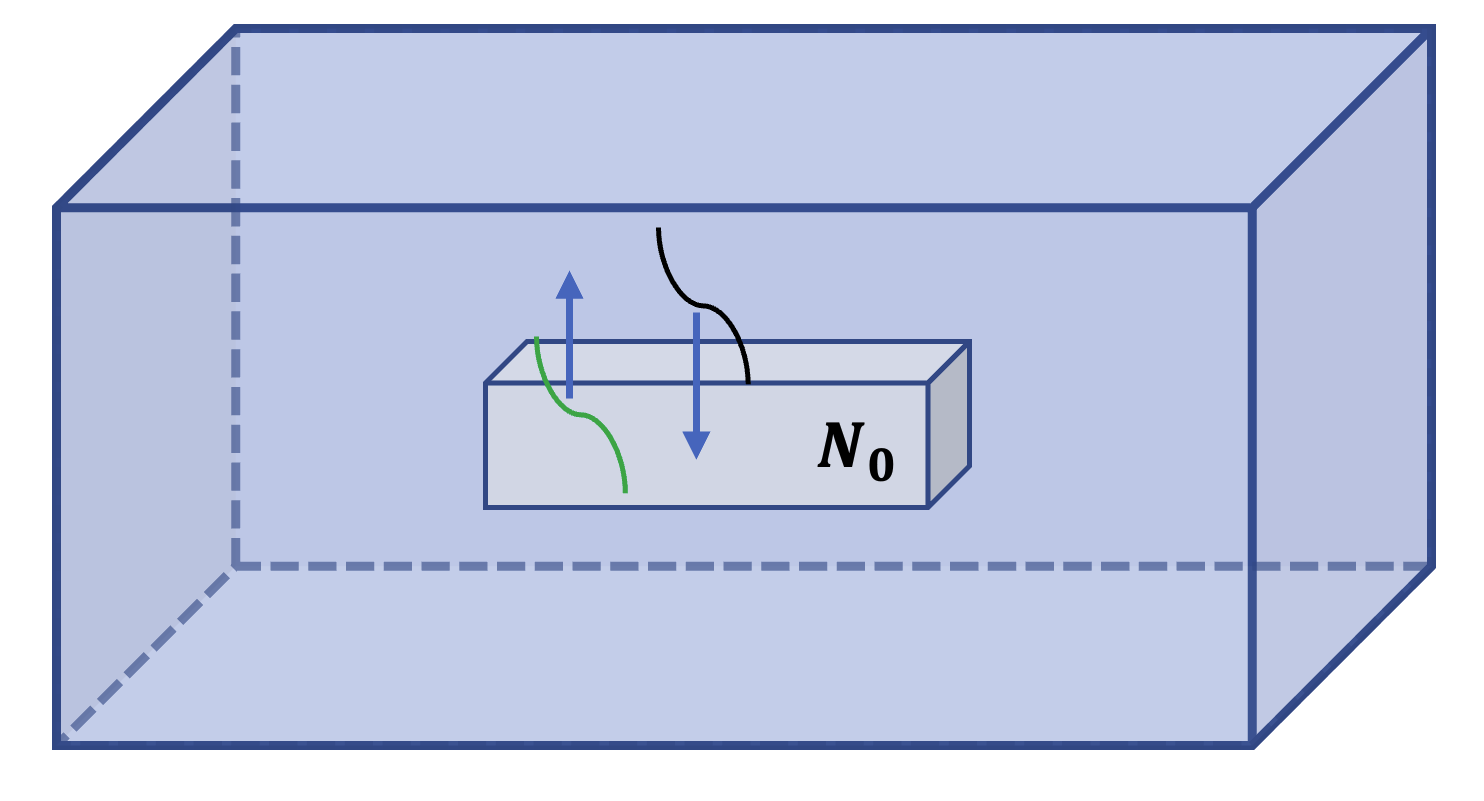
\includegraphics[width=0.5\linewidth]{figures/continuum_section.png}
    \caption{Sketch of the setting explained in the text. Polymers of different types may be exchanged with the surroundings, but the number of molecules $N_0$ inside the section of the particle simulation remains constant.}
    \label{fig:continuum_section}
  \end{figure}
This thesis is divided into three parts. All simulations are carried out using the \ac{SOMA} \cite{Schneider_soma} software package based on the \ac{SCMF} algorithm \cite{Daoulas06}. In the first part, as a first step towards boundary-driven particle simulations, the dynamics of noninteracting homopolymers are investigated. Specifically, a system is pushed away from equilibrium by introducing conversion zones at the boundary regions of the simulation box. This results in a diffusive current and allows the calculation of the collective diffusion coefficient of the system. To this end, the .\\
In the second part, a method to implement time-dependent boundary conditions in \ac{SOMA} is introduced using piecewise external fields. This method is exploited to obtain the bending modulus of diblock-copolymers.\\
In the final part, two approaches to dictate the composition at the boundaries according to a target field are introduced. The first approach is based on the conversion of macromolecule types and results in a non-convex optimization problem, as mentioned before. Two optimization algorithms are presented: the \ac{SA} algorithm and the \ac{SD} algorithm. In the second approach, the applied \ac{MC} scheme is modified in addition to the macromolecule type conversions to give a hybrid scheme. 




\chapter{Theory}

\section{Single-chain properties}

Since the collective dynamics of polymer mixtures can often be directly related to the single-chain properties, some selected aspects are briefly discussed here. The simplest model to describe a polymer chain is the ideal chain, for which any non-bonded interaction between monomers is neglected.

\subsection{Polymer types}

The properties of polymers depend greatly on the their molecular architecture. The simplest type of polymer is the homopolymer, which is a linear chain of monomers of the same monomer type. 

\begin{itemize}
    \item Show picture of different polymer types here
\end{itemize}

\subsection{The freely jointed chain}

The freely jointed chain model is an ideal model in which the chain is composed of $N$ segments of length $b_0\,,$ whose orientation vectors $\mathbf r_i$ ($b_0=|\mathbf r_i|$) can face in any direction and are completely independent from each other. Each segment therefore represents a step in a random walk \cite{Doi_edwards}. The chain configuration may be characterised by the end-to-end vector $\mathbf R$:

\begin{align}
    \mathbf R=\sum_{i=1}^{N}\mathbf r_i\,,
\end{align}

connecting the first and last segments. This is shown in \autoref{fig:ideal_chain}. Due to the completely random orientation, $\mathbf R$ has zero mean. A useful property to quantify the spatial extension of the chain is the mean square of $\mathbf R\,,$ which calculates to:

\begin{align}
    R_e^2\equiv \langle\mathbf R^2\rangle=Nb_0^2\,.
    \label{eq:Re}
\end{align}

\begin{figure}[h]
  \centering
  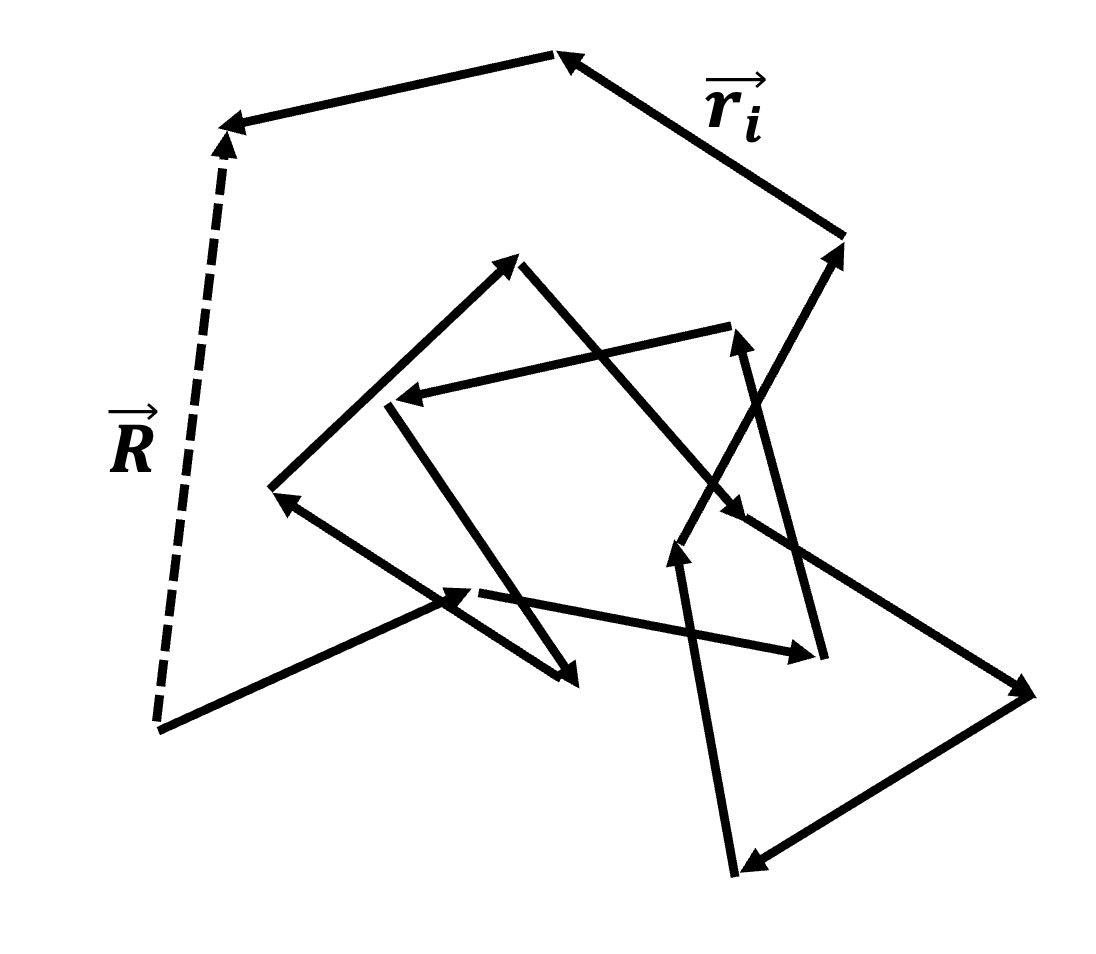
\includegraphics[width=0.5\linewidth]{figures/ideal_chain.png}
  \caption{Freely jointed chain.}
  \label{fig:ideal_chain}
\end{figure}

For large $N\,,$ $\mathbf R$ has a Gaussian distribution \cite{Rubin03}:
 
 
\begin{align}
    P(N,\mathbf R)=\left(\frac{3}{2\pi R_e^2}\right)^{3/2}\exp\left[-\frac{3\mathbf R^2}{2R_e^2}\right]\,,
\end{align}
 
 the freely jointed chain therefore converges towards the Gaussian chain. 
 
\subsection{Rouse model}

The Rouse model \cite{Rouse} is used to describe the dynamics of a Gaussian chain moving through a solvent. The stiff bonds are replaced by springs of root-mean-square size $b_0\,,$ through which a monomer interacts with its neighbours. The monomers experience a friction force with friction coefficient  $\zeta\,,$ and the total friction coefficient of the center of mass is:

\begin{align}
    \zeta_\mathrm R=N\zeta\,.
\end{align}

Within the Rouse model, the diffusion coefficient of the chain is computed as:

\begin{align}
    D_\mathrm R=\frac{k_BT}{\zeta_\mathrm R}=\frac{k_BT}{N\zeta}\,.
    \label{eq:d_rouse}
\end{align}

For an $n$-dimensional diffusion of a Brownian particle, the single chain diffusion constant is related to the mean squared displacement of the chain center of mass $g_3(t)$ by the Einstein relation \cite{einstein_1905}:

\begin{align}
    D&=\frac{g_3(t)}{2nt}\,, \label{eq:einstein_relation}\\
    g_3(t)&=\langle (\mathbf r_{cm}(t)-\mathbf r_{cm}(t_0))^2\rangle\,,\nonumber
\end{align}

where $\mathbf r_{cm}(t)$ is the center of mass position at time $t$ and $t_0$ is the time at which the measurement is started. The time in which a polymer diffuses a distance of the order of its size is called relaxation time $\tau_\mathrm R\,$:

\begin{align}
    \tau_\mathrm R\approx\frac{R_e^2}{D_\mathrm R}=\frac{\zeta}{k_BT}{NR_e^2}\,.
\end{align}

On time scales larger than $\tau_\mathrm R\,,$ the chain movement is only due to diffusion, while viscoelastic effects are observed at shorter time scales. 
 
 
\section{Polymeric mixtures}
Polymer mixtures consist of two or more chemically different polymer types. The mechanical and thermodynamic properties can vary greatly with several factors such as density, molecular weight and interactions between the polymers. This makes them desirable for manufacturing materials with tailored properties.\\
If the density is uniform everywhere, the mixture is called homogeneous. In a heterogeneous mixture, in contrast, the density is non-uniform, leading to visible boundaries which may have very different properties. This phenomenon is also called macro-phase separation. From an entropic viewpoint, mixing is always favored. However, energetic interactions between polymers may either favor or suppress mixing. Whether a mixture is homogeneous or heterogeneous, thus,  depends on the balance between entropy and energy \cite[S. 137]{Rubin03}.           

\subsection{Flory-Huggins Theory}

Whether mixing or phase separation will be favored can be predicted by determining the free-energy change associated with mixing the components. This free energy-change can be computed within the lattice model developed by Flory and Huggins \cite{Flory42}. Within the Flory-Huggins framework, no volume change is assumed upon mixing. With this assumption, it is convenient to represent the system on a lattice. A lattice site corresponds to the smallest molecular unit and every macromolecule takes up one or multiple lattice sites. Consider a binary mixture with $n_A$ polymers of species A and chain length $N_A$ and $n_B$ polymers of species B and chain length $N_B$. Let the total number of polymers be $n=n_A+n_B\,.$ The free energy of mixing per monomer $\Delta F_{mix}$ is then given by the Flory-Huggins equation of polymer solutions \cite[S. 143]{Rubin03}:

\begin{align}
  \frac{\Delta F_{mix}}{k_BT}=\frac{\phi}{N_A}\ln\phi+\frac{1-\phi}{N_B}\ln(1-\phi)+\chi\phi(1-\phi)\,.
  \label{eq:floryhuggins}
\end{align}

Here, $\phi=n_\mathrm AN_A/(n_\mathrm AN_A+n_\mathrm BN_B)$ is the monomer fraction of species A, $k_B$ is the Boltzmann constant, $T$ is the system temperature and $\chi$ is the Flory interaction parameter which characterizes the interaction between different polymer species and can be obtained from experiments. A positive value of $\chi$ opposes mixing while a negative value promotes it; knowing the value of $\chi$, therefore, allows us to qualitatively predict the phase separation behavior. For $\chi=0\,,$ \autoref{eq:floryhuggins} reduces to regular solution theory for an ideal gas of polymers with concentrations $\phi/N_A$ and $(1-\phi)/N_B\,.$  Note that so far, no space dependency of $\phi$ has been assumed. In the following discussion, a symmetric mixture with $N_A=N_B=N$ is assumed. To fully capture the complexity of the system, the Flory-Huggins model has to be extended to include spatial variations of $\phi$, which gives rise to the de Gennes-Flory-Huggins free-energy functional  \cite{deGennes80, Reister02}:


\begin{align}
  \frac{F[\phi]R_e^3}{k_BT\sqrt{\bar N}}=\int \mathrm{d}^3\mathbf{r}\left\{\phi\ln\phi+(1-\phi)\ln(1-\phi)+\chi N\phi(1-\phi)+k(\phi)[\nabla\phi]^2\right\}\,.
  \label{eq:flory_fctl}
\end{align}

Here, $\bar N=\left(nR_e^3/V\right)^2$ is the invariant degree of polymerization of the system with volume $V$. It is a measure of the number of neighboring chains a chain interacts with. The term proportional to $[\nabla\phi]^2$ is added to the free-energy density to ensure that unphysical, sharp changes in the local densities are penalized. The precise form of $k(\phi)$ depends on the strength of the parameter $\chi\,$. For small $\chi N\lesssim 5\,,$ one considers the \ac{WSL}. For large $\chi N\gtrsim10\,$ \cite{Semenov1996Dec}, the \ac{SSL} holds. In these two limits, the prefactor $k$ takes the following form \cite{Reister02}:

\begin{align}
  k_\mathrm{WSL}=\frac{R_e^2}{36\phi(1-\phi)}\,;\qquad k_\mathrm{SSL}=\frac{R_e^2}{24\phi(1-\phi)}\,.
\end{align}

\subsection{Phase separation}

The incompatibility between different monomer types causes diblock copolymers to self-assemble into interesting equilibrium morphologies. Besides the Flory-Huggins parameter $\chi N\,,$ the volume fraction $f$ of the $A$ block is crucial in determining the phase-separation behavior. Typical morphologies are shown in \autoref{fig:diblock_phasediagram} for increasing $f\,.$ The corresponding phase diagram may be obtained from experiments, or, numerically, from \ac{SCFT} computations \cite{matsen_copolymer}. The result of the latter is shown in \autoref{fig:diblock_phasediagram}.


\begin{figure}[h]
  \centering
  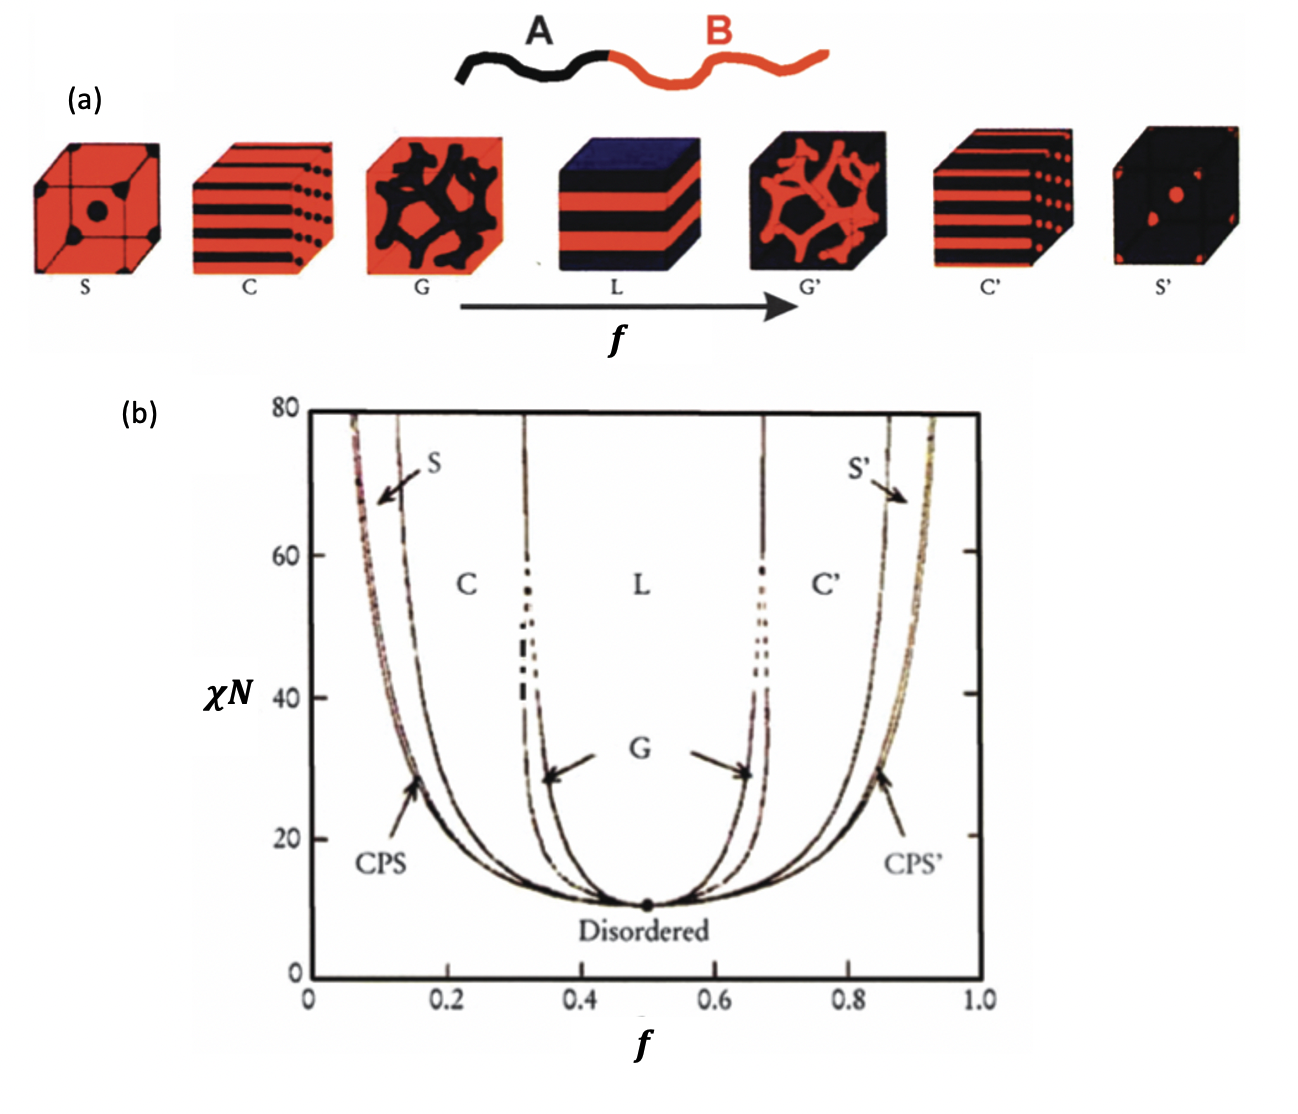
\includegraphics[width=0.8\linewidth]{figures/diblock_phasediagram.png}
  \caption{(a) Different equilibrium morphologies of diblock-copolymers for increasing values of $f\,.$ (b) $\chi N$-$f$ phase diagram. CPS stands for closely packed spheres, S for body-centered cubic spheres, C for hexagonally packed cylinders, G for bicontinuous gyroids and L for lamelale. Adapted from \cite{Mai_diblock_selfassembly}. }
  \label{fig:diblock_phasediagram}
\end{figure}

Below a critical value of $\chi N\approx 10.5\,,$ no structure formation occurs. This value is called the \ac{ODT}. At a fixed $\chi N> 10.5\,,$ several transitions between distinct, ordered morphologies occur for increasing $f\,.$ These transitions are called \acp{OOT}. The $A$ blocks first form closely packed spheres (CPS), which then transition into body-centered cubic spheres (S) and for even larger $f$ into cylindrical phases (C). Before reaching the lamellar phase (L), for not too large values of $\chi N\,,$ an additional phase is observed, the bicontinous gyroids (G). The same transitions occur in reversed order if $f$ is increased further beyond $0.5\,,$ where the characteristic morphologies are now assumed by the $B$ blocks.

\section{Collective diffusion}

Consider again a binary mixture of homopolymers with $N_A=N_B=N\,$. Since the number of polymers in the system is constant, the continuity equation holds:

\begin{align}
  \frac{\partial\phi}{\partial t}+\nabla\cdot\mathbf{J}_A=0\,.
  \label{eq:conti}
\end{align}

Here, $\mathbf{J}_A$ is the local current of polymer species A. Near equilibrium, one postulates a linear relation between $\mathbf{J}_A$ and the local chemical potential gradient $\nabla\mu_A$ \cite{deGennes80}. In the most general case, this relation is non-local in space and time. Assuming translational invariance in space and time, it reads \cite{erukhimovich1986nonexponential}:


\begin{align}
    \mathbf{J}_A(\mathbf{r},t)=-\int_{t'=-\infty}^t\mathrm d t'\int_V\mathrm d \mathbf{r'}\,\frac{\tilde\Lambda_A(\mathbf{r}- \mathbf{r'},t-t')}{k_BT}\nabla '\mu_A(\mathbf{r'},t')\,.
    \label{eq:linear_response}
\end{align}

The Onsager coefficient $\tilde\Lambda_A(\mathbf{r}- \mathbf{r'},t-t')$ relates the gradient of the chemical potential at position $\mathbf{r'}$ to a density flux at position $\mathbf r$ and also accounts for memory effects. It is often a good approximation to neglect the transmission of forces along the molecular backbone of the chain \cite{COOK1970297}. In this local approximation, the Onsager coefficient takes the simple form $\tilde\Lambda_A(\mathbf r,t)=\Lambda_A(\mathbf{r'},t')\delta(\mathbf r-\mathbf r')\delta(t-t')\,,$ so \autoref{eq:linear_response} simplifies to: 



\begin{align}
    \mathbf {J}_A=-\frac{\Lambda_A}{k_BT}\nabla\mu_A\,.
    \label{eq:current_local}
\end{align}


This approximation leads to a simple form of the Onsager coefficient for incompressible dynamics that will be derived in the following. 

%%  Derivation in Binder paper

% Following the discussion in the appendix of \cite{Binder83}, a continuity equation can be written down for each type individually:

% \begin{align}
%   \frac{\partial\phi_A}{\partial t}+\nabla\cdot\mathbf{J_A}=0\,; \qquad \frac{\partial\phi_B}{\partial t}+\nabla\cdot\mathbf{J_B}=0\,.
%   \label{eq:conti_ab}
% \end{align}

% With the additional assumption of incompressibility, e.g. $\rho(\mathbf{r},t)\equiv\phi_A(\mathbf{r},t)+\phi_B(\mathbf{r},t)=1$ everywhere for all times, the continuity equation for the total density $\rho$ separates into two distinct equations:

% \begin{align}
%   \frac{\partial}{\partial t}(\phi_A+\phi_B)=0\,; \qquad \nabla\cdot (\mathbf{J_A}+\mathbf{J_B})=0  \,.
% \end{align}

% This implies that $\mathbf{J_A}=-\mathbf{J_B}\,,$ which simply reflects the condition of incompressibility: for a bead of type A to move, a bead of type B has to take its place and vice-versa. The Onsager relations are then
% \begin{subequations}
%   \begin{align}
%     \mathbf{J_A}&=-\frac{\Lambda_{\mathrm{AA}}}{k_BT}\nabla\mu_A\,,\\
%     \mathbf{J_B}&=-\frac{\Lambda_{\mathrm{BB}}}{k_BT}\nabla\mu_B\,,
%     \label{eq:current_onsager}
%   \end{align}
% \end{subequations}


% where $\Lambda_\mathrm{AA}$ and $\Lambda_\mathrm{BB}$ are the diagonal elements of the matrix of Onsager coefficients, which is assumed to be diagonal. Since $\mu_A$ and  $\mu_B$ are not independent variables, their difference $\Delta\mu=\mu_A-\mu_B$ is considered instead. The goal is now to relate $\Delta\mu$ to the current $\mathbf J(\mathbf r,t)=\mathbf {J_A}(\mathbf r,t)=-\mathbf {J_B}(\mathbf r,t)\,.$ From \autoref{eq:current_onsager}, it is easily seen that

% \begin{align}
%   \nabla(\mu_A-\mu_B)&=-k_BT\left (\mathbf{J_A}\Lambda_{\mathrm{AA}}^{-1} - \mathbf{J_B}\Lambda_{\mathrm{BB}}^{-1}\right )\nonumber\\
%   &=-k_BT\left (\Lambda_\mathrm{AA}^{-1}+\Lambda_\mathrm{BB}^{-1}\right )\mathbf{J}
% \end{align}

% and therefore

% \begin{align}
%   \mathbf J=-\frac{1}{k_BT}\left (\Lambda_\mathrm{AA}^{-1}+\Lambda_\mathrm{BB}^{-1}\right )^{-1}\nabla(\mu_A-\mu_B)\,.
% \end{align}

% The Onsager coefficient that relates $\mathbf{J}$ to the local chemical potential difference is identified as $\Lambda^{-1}=\Lambda_\mathrm{AA}^{-1}+\Lambda_\mathrm{BB}^{-1}\,.$ By relating the currents in \autoref{eq:current_onsager} to the single chain diffusion coefficients $D_A$ and $D_B\,,$ the Onsager coefficients may be identified as $\Lambda_\mathrm{AA}=N_\mathrm AD_A\phi$ and $\Lambda_\mathrm{BB}=N_\mathrm BD_B(1-\phi)\,.$ For a symmetric mixture with $N_A=N_B\equiv N $ and $D_A=D_B\equiv D\,,$ the Onsager coefficient corresponding to $\Delta\mu$ becomes


% \begin{align}
%   \Lambda=DN\phi(\mathbf{r})(1-\phi(\mathbf{r}))\,.
%   \label{eq:onsager}
% \end{align}


% This result has also been derived by de Gennes \cite{deGennes80}.\\


%% Alternative derivation in de Gennes paper


Following the discussion in the appendix of \cite{deGennes80}, consider a mixture of polymer chains with densities $\phi_A$ and $\phi_B\,.$ Incompressibility, e.g. $\phi_A+\phi_B=1\,,$ is enforced by introducing an additional, repulsive potential $U$ to the chemical potential, so from \autoref{eq:current_local} one obtains:



\begin{subequations}
  \begin{align}
    \mathbf{J}_A&=-\Lambda_A\nabla [(\mu_A + U)/k_BT]\,,\\
    \mathbf{J}_B&=-\Lambda_B\nabla [(\mu_B + U)/k_BT]\,.
  \end{align}
  \label{eq:current_onsager}
\end{subequations}

Due to the incompressibility, the total current $\mathbf J_{tot}=\mathbf{J}_A+\mathbf{J}_B$ must have zero divergence, which in one dimension means $\mathbf J_{tot}\equiv J_{tot}\mathbf{e_x}=\mathrm{const}\,.$ From the Galilei invariance of the system, we can simply choose $J_{tot}=0\,.$ From this condition, $U$ can be calculated explicitly:

\begin{align}
  U=(\Lambda_A\mu_A+\Lambda_B\mu_B)/(\Lambda_A+\Lambda_B)\,.
\end{align}

Since one of the currents is redundant, write $J\equiv J_A\,.$ From \autoref{eq:current_onsager}, obtain:

\begin{align}
  J=-\frac{\Lambda}{k_BT}\nabla(\mu_A - \mu_B)\equiv -\frac{\Lambda}{k_BT}\nabla\mu\,,
\end{align}

where $\Lambda=\Lambda_A\Lambda_B/(\Lambda_A+\Lambda_B)$ and $\mu$ is the exchange chemical potential. In the limit of no interactions, the mixture can be considered as an ideal gas, so $\Lambda_i=D_i\phi_i$ for $i=A, B\,.$ For $D_A=D_B\equiv D\,,$ this yields:

\begin{align}
  \Lambda=D\phi(\mathbf{r})(1-\phi(\mathbf{r}))\,.
  \label{eq:onsager}
\end{align}
This approximation is frequently used in the literature for the sake of computational efficiency \cite{Fraaje97,deGennes80,Binder83}. It corresponds to a local coupling in which monomers move like the center of mass, therefore it does not account for the connectivity of the monomers along the backbone of the chain. 

\section{Single chain in mean field simulations}


% First option following http://dx.doi.org/10.1063/1.2364506

Although the model used in this thesis provides a high flexibility in molecular architectures, the following discussion is restricted to symmetric  AB-diblock copolymers in a volume $V$ at temperature $T$ for simplicity. We consider the partition function \cite{Daoulas06}:

\begin{align}
    \mathcal{Z}\propto\frac{1}{n!}\int{\prod_{i=1}^n\mathcal{D}[\mathbf r_i(s)]\mathcal P_0[\mathbf r_i(s)]\exp\left(\frac{-\mathcal H_{\text{nb}}[\hat\phi_A,\hat\phi_B]}{k_BT}\right)}\,,
    \label{eq:partition_punction}
\end{align}

where $\mathbf r_i(s)$ is the position of segment $s$ from molecule $i\,.$ The factor $\int\mathcal{D}[\mathbf r_i(s)]\equiv \int\prod_sd^3\mathbf r_i(s)$ integrates over the conformation space of molecule $i\,.$ Conformations are weighted by a Boltzmann factor $P_0[\mathbf r_i(s)]\propto\exp\left(-\mathcal H_{\text{b}}[\mathbf r_i(s)]/k_BT\right)$ that involves the bonded interactions in the abscence of any intermolecular interactions. The bonded interactions $\mathcal H_{\text{b}}[\mathbf r_i(s)]$ are modeled by harmonic potentials, which is appropriate for Gaussian polymers. The discretized form reads:

\begin{align}
    \frac{\mathcal H_b[\mathbf r_i(s)]}{k_BT}=\sum_{s=1}^{N-1}\frac{3(N-1)}{2R_{e0}^2}[\mathbf r_i(s)-\mathbf r_i(s+1)]\,.
\end{align}

Here, $R_{e0}^2$ is the mean squared end-to-end distance of the polymer in the absence of non-bonded interactions. The non-bonded interactions $\mathcal H_\text{nb}$ in \autoref{eq:partition_punction} depend on the local particle densities $\hat\phi_A$ and $\hat\phi_B\,,$ which are defined on a cubic grid with spacing $\Delta L$ in the discretized model, the total number of cells is $N_{cells}=V/(\Delta L)^3\,.$ The densities are obtained by summing over all beads and assigning them to their according cell:

\begin{align}
    \hat\phi_{\alpha,m}=\sum_{i=1}^n\sum_{s=1}^N\Pi(\mathbf r_i(s),\mathbf c_m)\gamma_\alpha(s)\,,
    \label{eq:normalized_densities}
\end{align}

where $\gamma_\alpha(s)$ assigns the segments to their respective types: it is one if segment $s$ is of type $\alpha\,,$ and zero otherwise. $\Pi(\mathbf r_i(s),\mathbf c_m)$ is the characteristic function of the grid cell centered at $\mathbf c_m\,.$ The non-bonded interactions are modeled by the following discretized excess free energy functional:

\begin{align}
    \frac{\mathcal H_\text{nb}[\hat\phi_A,\hat\phi_B]}{k_BT}=\frac{\rho_0\Delta L^3}{N}\sum_{m=1}^{N_{cells}}\left(\frac{\kappa_0 N}{2}[\hat\phi_{A,m}+\hat\phi_{B,m}-1]^2-\frac{\chi_0 N}{4}[\hat\phi_{A,m}-\hat\phi_{B,m}]^2\right)\,.
    \label{eq:nonbonded_discretized}
\end{align}

where $\rho_0=\frac{nN}{V}$ is the average monomer density. The first term in the sum penalizes deviations of the total density from unity, and therefore controls the extent of density fluctuations with the control parameter $\kappa_0\,.$ The second term enforces the repulsion of monomers of different types with the control parameter $\chi_0\,.$ It should be emphasized that $R_{e0}^2\,,$ $\kappa_0N$ and $\chi_0N$ are coarse-grained parameters. The spatial discretization and the presence of density fluctuations give rise to deviations of the inverse compressibility $\kappa N\,,$ the Flory-Huggins parameter $\chi N$ and the mean squared end-to-end distance $R_e^2$ from the corresponding model parameters. For most systems, these deviations are small. For this reason, the physical quantities and model parameters will be used interchangeably in the following. \\
Instead of using direct \ac{MC} simulations, it is useful to look at typical scales of the bonded and non-bonded interactions. The bonded interactions are typically much stronger and less computationally expensive. For a given $\chi N\,,$ the typical ratio of bonded to non-bonded forces scales like $N^{3/2}$ \cite{Mueller_daoulas11}. Furthermore, the variations of the non-bonded interactions are much slower. The key idea behind \ac{SCMF} simulations is to exploit these scaling differences to replace the explicit non-bonded interactions by quasi-instantaneous external fields $\omega_{\alpha,m}$:


\begin{align}
    \omega_{\alpha,m}&=\frac{1}{k_BT\rho_0\Delta L^3}\frac{\partial \mathcal H_{\text{nb}}}{\partial \hat\phi_{\alpha,m}}\,,\nonumber \\
    \omega_{A,m}&=\kappa N\left(\hat\phi_{A,m}+\hat\phi_{B,m}-1\right)-\frac{\chi N}{2}\left(\hat\phi_{A,m}-\hat\phi_{B,m}\right)\,,
    \label{eq:calc_omegafields}
\end{align}

and similarly for $\omega_{B,m}\,.$ This way, \autoref{eq:nonbonded_discretized} is rewritten to:

\begin{align}
    \frac{\mathcal H_\text{nb}^{\text{SCMF}}[\hat\phi_A,\hat\phi_B]}{k_BT}=\frac{\rho_0\Delta L^3}{2N}\sum_{m=1}^{N_\text{cells}}\omega_{A,m}\hat\phi_{A,m}+\omega_{B,m}\hat\phi_{B,m}\,.
\end{align}

The actual \ac{SCMF} algorithm consists of two steps. First, the external fields are computed according to \autoref{eq:calc_omegafields}. Subsequently, they are kept constant over a short duration during which a \ac{MC} scheme is used to update the particle positions. A trial move is proposed according to a predefined rule and accepted according to the Metropolis-Hastings criterion \cite{metropolis}:

\begin{align}
    p_{\text{acc}}=\min\left\{1\,,\exp\left(-\frac{\Delta E}{k_BT}\right)\right\}\,,
    \label{eq:metropolis_mc}
\end{align}

where $\Delta E=\Delta\mathcal H_b+\Delta\mathcal H_{\text{nb}}^{\text{SCMF}}$ is the energy change associated with the move. After a predefined number of \ac{MC} steps, the external fields are recalculated from the current densities and the procedure is repeated. The independent time evolution of polymers thanks to the quasi-instantaneous field approximation allow for an efficient implementation on parallel computers. The accuracy of the \ac{SCMF} algorithm depends on the update frequency of the external fields and the parameter

\begin{align}
    \epsilon=\frac{1}{\sqrt{N\bar N}}\left(\frac{b_0}{\Delta L}\right)^3\,,
\end{align}

which needs to be small \cite{Schneider_soma}.

\section{Smart Monte Carlo Move}

Traditionally, a \ac{MC} trial move would consists of a displacement of each particle by a random, normalized, Gaussian distributed vector $\Delta\mathbf R\,.$ The freedom of choice of this trial move in the original Metropolis Algorithm \cite{metropolis} can be exploited to achieve higher acceptance rates. The \ac{SMC} move introduces an additional term proportional to the bonded forces $\mathbf{F}_i(\mathbf r)$ \cite{smc, mueller_deltat}:

\begin{align}
    \mathbf{r'}_i(s)=\mathbf{r}_i(s)+\mathbf{F}_i(\mathbf r)\Delta A+\Delta\mathbf R\,,
\end{align}

which is simply and Euler integration with time step $\Delta t=\zeta_0\Delta A\,.$


% Second option following http://dx.doi.org/10.1063/1.2364506
% Might be better because it is simpler and at the same time more general

% Within the soft, coarse grained model employed here, in principle, a great variety of molecular architectures can be implemented. For this reason, the term \enquote{macromolecule} will be frequently used in the following instead of \enquote{polymer}. The pairwise interaction energy associated with a bond $b$ of a molecule $m$ is $V_{m,b}(\mathbf r)\,.$
% Macromolecules, which are defined as a group of particles linked together by bonds, can take one of $m_t$ different molecular architectures. These architectures define the bond topology. The total bonded interactions are obtained by summation over all interactions of bonds $b$ in every molecule $m\,$: 

% \begin{align}
%     \frac{\mathcal H_B}{k_BT}=\sum_{m\in \text{\{mol\}}}\sum_{b\in {\text{\{bonds\}}}_m}V_{m,b}(\mathbf r)\,,
% \end{align}

% where $V_{m,b}(\mathbf r)$ is the interaction energy of a single bond and $\mathbf r$ denotes the distance vector between the two bond partners. Motivated by a coarse-graining of Gaussian chains, it is chosen as a harmonic potential:

% \begin{align}
%     V_{\text{harm}}(\mathbf r)=\frac{1}{2}k_0\mathbf r^2\,,
% \end{align}

% where $k_0$ is the spring constant. Each particle has one of $n_t$ different types, which dictate the non-bonded interactions. As done in the Self-Consistent Field Theory (SCFT) for multi-component polymer melts, these are defined as excess free energy functionals that depend on the local, normalised densities $\hat\phi_i(\mathbf r)$ with $i=0,\dots,n_t\,.$ These densities are defined on a cubic grid with linear spacing $\Delta L\,$:

% \begin{align}
%     \hat\phi_i(c)=\frac{1}{\Delta L^3\rho_0}\sum_{j\in\text{beads}}\Pi_c(\mathbf r_j)\delta_{\text{type}(j),i}\,,
%     \label{eq:density_grid}
% \end{align}

% where $\rho_0$ denotes the average number density of particles in the system and $\Pi_c(\mathbf r_j)=1$ if the $j$th bead is in cell $c$ and $\Pi_c(\mathbf r_j)=0$ otherwise. The non-bonded interactions are then defined as:

% \begin{align}
%     \frac{\mathcal H_{\text{nb}}[\{\hat\phi_i\}]}{k_BT}=\frac{\rho_0\Delta L^3}{N}\sum_{c\in\{\text{cells}\}}\left(\mathcal K_\text{fluc.}[\{\hat\phi_i(c)\}]+K_\text{inter.}[\{\hat\phi_i(c)\}]\right)\,.
% \end{align}

% Fluctuations of the total density are controlled by the term: 

% \begin{align}
%     \mathcal K_\text{fluc.}[\{\hat\phi_i(c)\}]=\frac{\kappa N}{2}\left(\sum_{i=0}^{n_t-1}\hat\phi_i(c)-1\right)^2\,,
% \end{align}

% where $\kappa$ is a model parameter that controls the compressibility. The second term,

% \begin{align}
%     \mathcal K_\text{inter.}[\{\hat\phi_i(c)\}]=-\sum_{i\neq j}\frac{\chi_{ij}N}{4}\left(\hat\phi_i(c)-\hat\phi_j(c)\right)^2\,,
% \end{align}

% controls the incompability between different types. The matrix $\chi_{ij}$ is a generalisation of the Flory-Huggins parameter to multi-component systems. The SCMF algorithm now exploits the fact that the non-bonded interactions are typically significantly weaker than the bonded interactions and temporal variations are slow. Instead of calculating them explicitly, they are approximated by quasi-instantaneous external fields, $\omega_i(c)\,,$ which are calculated as:

% \begin{align}
%     \omega_i(c)&=\frac{1}{k_BT\rho_0\Delta L^3}\frac{\partial \mathcal H_{\text{nb}}}{\partial \hat\phi_i(c)} \nonumber\\
%     &=\kappa\left(\sum_{i=0}^{n_t-1}\hat\phi_i(c)-1\right)-\sum_{k\neq i}\frac{\chi_{ik}}{2}\left(\hat\phi_i(c)-\hat\phi_j(c)\right)\,.
%     \label{eq:calc_omegafields}
% \end{align}


% In the SCMF algorithm, the particle  configuration at the current time step is used to compute the external fields, $\omega_i\,,$ given by  \autoref{eq:density_grid} and \autoref{eq:calc_omegafields}. Subsequently, the particles are subjected to these external fields and displaced according to a MC scheme, which involves the bonded interactions $\mathcal H_B$ and the SCMF interaction with the external field: 

% \begin{align}
%     \frac{\mathcal H_{\text{nb}}^\text{SCMF}}{k_BT}=\sum_{i=0}^{n_t-1}\sum_{c\in\{cells\}}\Delta L^3\rho_0\hat\phi_i(c)\omega_i(c)=\sum_{j\in\{beads\}}\omega_{\text{type}(j)}(c_j)\,,
% \end{align}

% where $c_j$ denotes the cell of particle $j\,.$


% \section{Smart Monte Carlo move}

% \begin{itemize}
%     \item to be extended
% \end{itemize}
% The friction from the Rouse model can be incorporated into MC simulations by using a Smart Monte Carlo (SMC) scheme \cite{SMC}. The particle positions are proposed according to:

% \begin{align}
%     \mathbf{r}_i'(s)=\mathbf{r}_i(s)+\frac{\Delta t}{\zeta}\mathbf F_i(\mathbf r)+\Delta \mathbf r\,,
% \end{align}

% where $\Delta \mathbf r$ is from the usual MC algorithm and $\mathbf F_i(s)$ is the bonded force acting on the segment. $\Delta t$ is the time step of the simulation and $\zeta$ controls the segmental friction. The value of $\Delta t\,,$ that maximizes the MC acceptance rate, was found to be $\Delta t=0.17(\zeta R_e^2/Nk_BT)\,$ \cite{mueller_deltat}.


\section{Discrete optimization}

As will be shown in \autoref{chap:polyconversion}, applying non-periodic boundary conditions in \ac{SCMF} simulations by converting molecule types leads to a discrete optimization problem. This type of problem involves finding the best configuration $S^*$ out of a finite set $\Omega$ of possible configurations, e.g., the one that minimizes a certain loss function $f(S)\,,$ where $S$ is an arbitrary configuration. $\Omega$ is often called \textit{search space}. In this thesis, only minimization problems are considered. Maximization is completely analogous. These problems are often NP-complete \cite{gary1979computers}, and, therefore, designing efficient algorithms is very difficult. One usually distinguishes between convex and non-convex optimization problems. Convex problems only have a single, global minimum. The optimal solution can be found efficiently by applying a greedy algorithm. In each iteration step, a new solution is proposed and accepted only if it leads to a reduction in the loss function \cite{cormen01introduction}. It therefore gradually moves towards the global optimum. If the problem is non-convex, then there exist multiple local minima in which the greedy algorithm is likely to become trapped. 

\section{Simulated Annealing}
\label{sec:sa}
\ac{SA} \cite{simulated_annealing} is a heuristic algorithm that is frequently used to find at least an approximate optimum for a non-convex discrete optimization problem. It is inspired by the annealing process in metallurgy, in which the crystallization of a material is enhanced by heating it up to a high temperature and letting it cool down slowly \cite{sa_applications}. For this, a temperature parameter $T$ is introduced. It starts from an initially high temperature $T_0$ which is reduced according to a predefined rule

\begin{align}
    T_{k}=g(k)\,,
    \label{eq:cooling_schedule}
\end{align}

until a minimal temperature $T_f$ is reached. Initially, the algorithm makes an initial guess $S_0\in \Omega$ for the optimal solution. At each temperature, a new solution $S^*$ is created from the current solution $S$ according to a specific generation rule. The new solution is accepted with a probability given by the Metropolis-Hastings criterion, similar to \autoref{eq:metropolis_mc}:

\begin{align}
    p(S\rightarrow S^*)=\min\left\{1\,,\exp\left(-\frac{f(S^*)-f(S)}{T}\right)\right\}\,.
\end{align}

Instead of proposing only a single neighboring solution at each temperature, multiple trials are also possible. This is essentially the same as performing a \ac{MC} simulation while lowering the temperature. Much like atoms in a solid have larger degrees of freedom at high temperatures, new solutions have a higher probability of being accepted at high temperatures. Accepting worse solutions leads to a good \textit{exploration} of the search space and it can prevent the algorithm from becoming trapped in a local minimum. As the temperature is decreased, the algorithm transitions towards an \textit{exploitation} phase, in which mostly only better solutions are accepted.\\
The efficiency of \ac{SA} and the quality of the optimum depends greatly on the applied cooling schedule. Under a certain set of conditions, the algorithm is guaranteed to converge if the cooling is logarihmic \cite{hajek_sa}, e.g., 

\begin{align}
    T_k=\frac{d^*}{\log(k+1)}\,,
\end{align}

where $d^*$ is the maximum depth of all local minima excluding the global minimum. This theoretical result is not very useful, since $d^*$ is difficult to determine and logarithmic cooling is much too slow for practical use. The cooling schedule must be chosen in order to achieve a good trade-off between computational efficiency and quality of the optimum. There is no general choice for $T_0\,,$ $T_f$ and $g(k)$ in \autoref{eq:cooling_schedule} that yields good results for any problem. Rather, the parameters have to be tuned empirically to the problem at hand. This is further complicated by the fact that, in most cases, no a priori guess can be made for the value of $f$ at the global minimum.

\chapter{Simulation technique}


To simulate the collective dynamics, a coarse-grained model of the polymers is employed. Within this model, several monomeric repeat units are grouped into \textit{beads}, which allows for an efficient numerical implementation. Nevertheless, in this study, the terms \enquote{bead} and \enquote{monomer} will be used interchangeably. Each macromolecule is assigned one of $m_t$ possible architectures upon initialization. The architecture describes the bead types and bond topology of the macromolecule. Other than simple homopolymers, more complex bond topologies like copolymers, star polymers and rings are possible. A great variety of universal properties of polymeric materials on mesoscopic length scales is accurately captured by coarse-grained models \cite{Baschnagel03}.\\
The software package that is used for the numerical calculations, \ac{SOMA}, uses a combination of the described coarse-grained model and the \ac{SCMF} algorithm \cite{Daoulas06}. Unlike the widely used \ac{SCFT}, the \ac{SCMF} method includes fluctuation effects which are required to accurately describe certain systems and effects, e.g. dilute polymer solutions, the vicinity of phase transitions, or polymeric microemulsions \cite{Bates97, Mueller02, Schmid03}. The interactions are fully described by three coarse-grained parameters: the average mean squared end-to-end distance $R_{e}^2$ of a chain in the absence of non-bonded interactions, the inverse thermal compressibility $\kappa_0 N$ and the incompatibility between different bead types $\chi_0 N$. The term \enquote{soft} in \ac{SOMA} relates to the soft nature of the non-bonded interactions, which arises from the systematic coarse-graining and allows for an overlap of beads \cite{Mueller11soft}. As mentioned before, the enormous benefit of the \ac{SCMF} algorithm is that the chains are decoupled, making it possible to implement it effectively on parallel machines. For this, the \ac{MPI} standard is employed. Each molecule is assigned to a specific \ac{MPI} rank and the densities are computed according to \autoref{eq:normalized_densities}. \ac{SOMA} also supports parallelization on shared-memory systems using the OpenMP standard as well as the use of accelerators like Nivida \acp{GPU} \cite{Schneider_soma} using the OpenACC standard. For the particle propagation, a \ac{SMC} scheme is employed that uses the strong bonded forces to propose a trial displacement resembling Brownian motion and produces Rouse-like dynamics \cite{Pangali78,Rossky78}. Another important feature of \ac{SOMA} is the conversion of macromolecules to different types of the same bond architecture, but with different bead types. This allows for the simulation of chemical reactions, or, as used in this thesis, to generate a flux. \\
The conversion-based-target-composition plugin is implemented to read in target composition fields and optimize the polymer type configurations, as explained in \autoref{chap:polyconversion}. The identification of the target polymers, as well as the matrices $\tilde q$ and $\tilde n\,,$ as explained in Algorithms \ref{alg:get_flip_candidates}-\ref{alg:get_cell_numbers}, can be performed in parallel using OpenACC. The actual optimization process is inherently sequential and parallelization is thus impossible. Based on the initial temperature $T_0\,,$ an optimization algorithm is chosen: if $T_0>0\,,$ \ac{SA} will be performed. Otherwise, the \ac{SD} algorithm is employed. The interaction part of the quasi-instantaneous external fields is modified as explained in \autoref{sec:hybrid}


\chapter{Collective diffusion of symmetric homopolymers}
\label{chap:colldiff}

To describe the collective diffusion behavior of polymer mixtures, the most important quantity is the Onsager coefficient. In this section, the simple case of an effectively one-dimensional current is investigated by simulation of a binary homopolymer mixture in a confined simulation box. The form \autoref{eq:onsager} for the Onsager coefficient is obtained. 

\section{Reference system}

The collective diffusion properties of non-interacting homopolymers with $N_A=N_B=N$ and $\chi=0$ are investigated. As a reference system, a simulation box with $n_A=n_B=5000$ polymers and dimensions $L_x\times L_y\times L_z=9.75\times3\times3\,R_e^3$ is used, so the invariant degree of polymerization is $\sqrt{\bar{N}}\approx 114\,$. The spatial discretization is $\Delta L=0.125\,R_e\,$.  Periodic boundary conditions are applied in the lateral $y$ and $z$ directions, whereas impenetrable walls are applied in the $x$ direction. Initially, the polymers are distributed homogeneously in the system. To stimulate a flux in a \ac{NESS}, conversion zones of width $d=0.25\,R_e$ are introduced close to the walls. In each time step, if the center-of-mass coordinate $\mathbf r_{cm}$ of a polymer of type A lies in the left conversion zone, it is converted to type $B$ with probability $p(A\rightarrow B)=r\,$. Analogously, conversion from $B$ to $A$ takes place in the right conversion zone with the same probability $r\,$. The current $\mathbf J$ is measured by tracking the number of polymer conversions. The simulation setup is depicted in \autoref{fig:simulation_box}. \\
The computation of the transport properties is complicated by boundary effects, such as a steep density drop close to the hard walls, which is of entropic origin. As a result, the densities defined in \autoref{eq:normalized_densities} do not exactly sum up to one in the bulk. In \autoref{fig:density_drop}, it can be seen that the total density is about $1.01$ in the bulk and drops to $0.65$ in the cells that border the walls directly.

\begin{figure}[H]
  \centering
  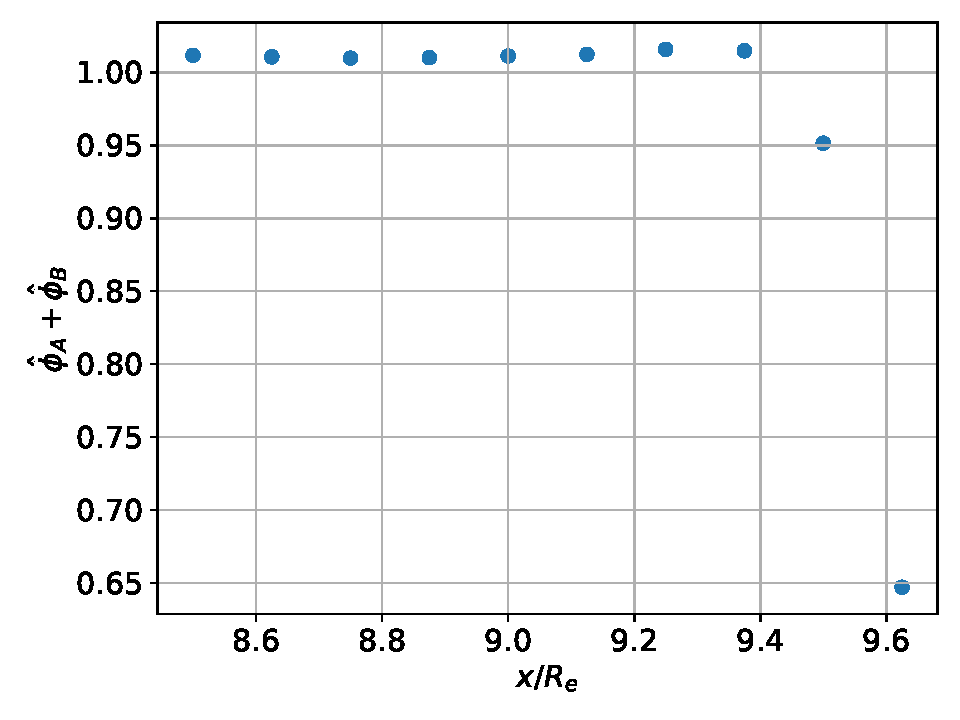
\includegraphics[width=0.6\linewidth]{figures/density_drop.pdf}
  \caption{One dimensional profile of the total density.}
  \label{fig:density_drop}
\end{figure}

Furthermore, chains whose center of mass lies in the conversion zone may extend far beyond that zone. The range of these effects is approximated as $R_e$ and measurements are only taken in the region where the effects are negligible. The total densities are re-normalized by dividing by the average value in the bulk.


\begin{figure}[h]
  \centering
  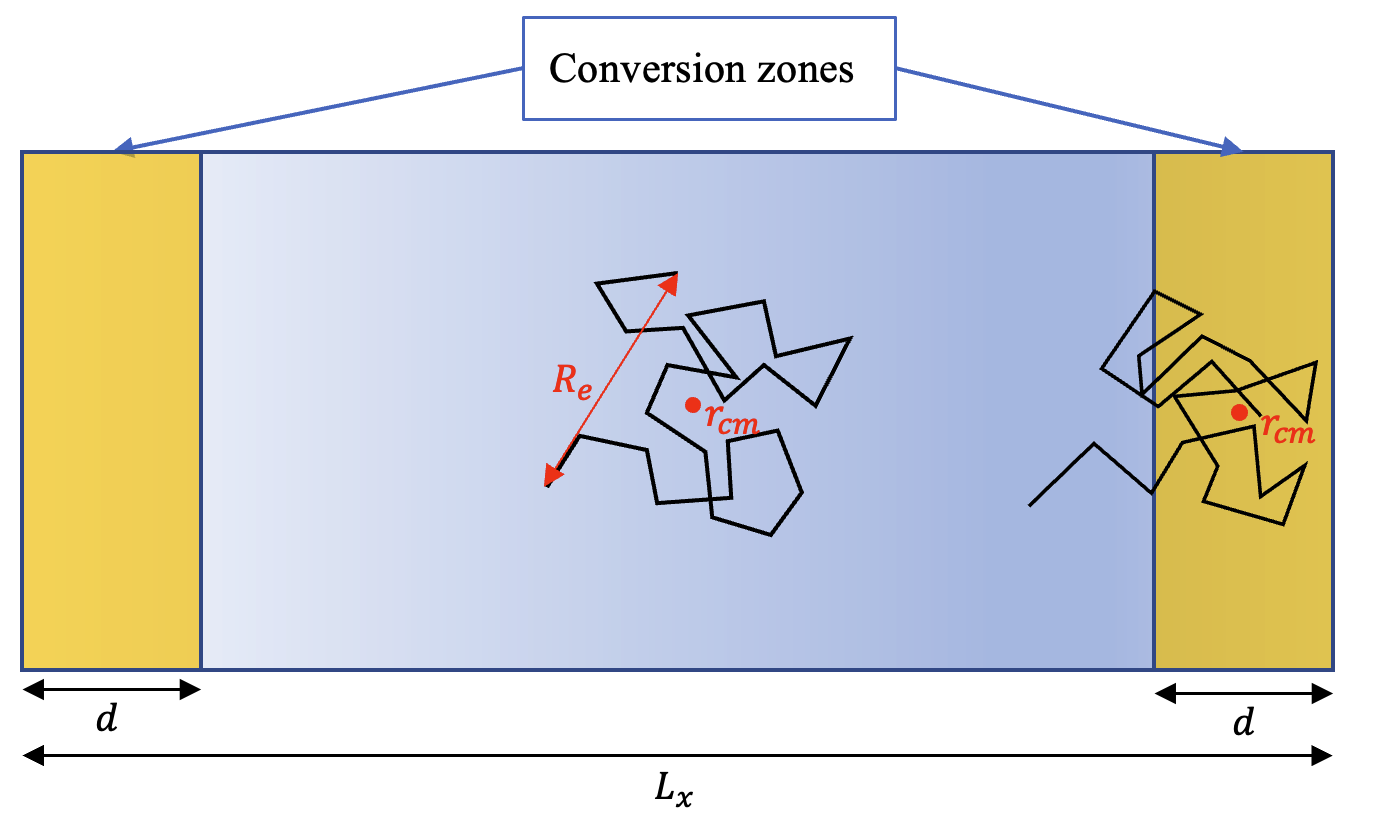
\includegraphics[width=0.7\linewidth]{figures/simulation_box.png}
  \caption{Simulation setup. For clarity, the conversion zones are not to scale and no distinction between polymer types is made.}
  \label{fig:simulation_box}
\end{figure}


\section{Collective diffusion coefficient}
\label{sec:colldiff}

Due to the periodic boundary conditions and the spatial homogeneity in the lateral directions, the system can effectively be described in one dimension. The density profile for $r=1.0$ is shown in \autoref{fig:density_profile}.

\begin{figure}[h]
  \centering
  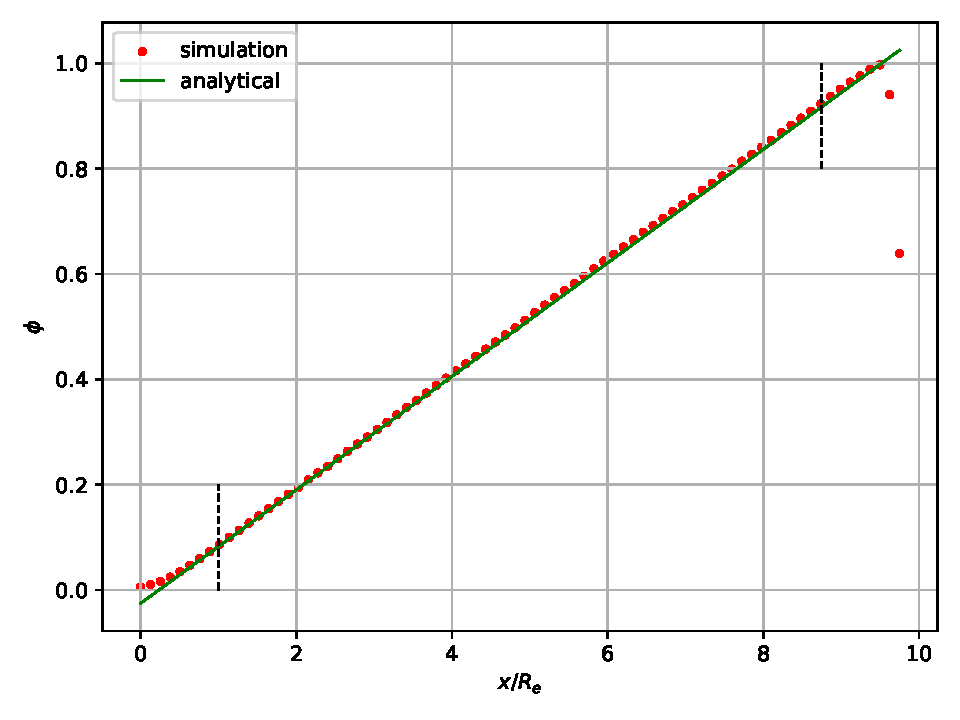
\includegraphics[width=0.6\linewidth]{figures/density_coll_diff.pdf}
  \caption{Steady-state density profile for $r=1.0$ averaged over $y$ and $z\,$. The analytical curve corresponds to \autoref{eq:density_profile_ana}. The black lines mark the region that is estimated to be affected by boundary effects.}
  \label{fig:density_profile}
\end{figure}

Outside of the range of the boundary effects, the density profile is very well represented by a linear function. The chemical potential is obtained by taking the functional derivative $\frac{\delta F}{\delta\phi}$ of \autoref{eq:flory_fctl}. Since $\chi=0\,$, no phase separation occurs and the local density differences are entirely due to the dynamics. Assuming the WSL, the chemical potential becomes:


\begin{align}
  \frac{\mu R_e^3}{\sqrt{\bar N} k_BT}&=\ln\phi-\ln(1-\phi)-\frac{R_e^2}{18\phi(1-\phi)}\phi''\nonumber \\ &+\left[\frac{R_e^2(1-2\phi)}{36\phi^2(1-\phi)^2}\right]\phi'^2\,,
  \label{eq:mu_flory}
\end{align}

where the dashes denote derivatives with respect to $x\,.$ The resulting chemical potential profile is shown in \autoref{fig:chemical_potential}.



\begin{figure}[h]
  \centering
  \begin{subfigure}[b]{0.45\textwidth}
      \centering
      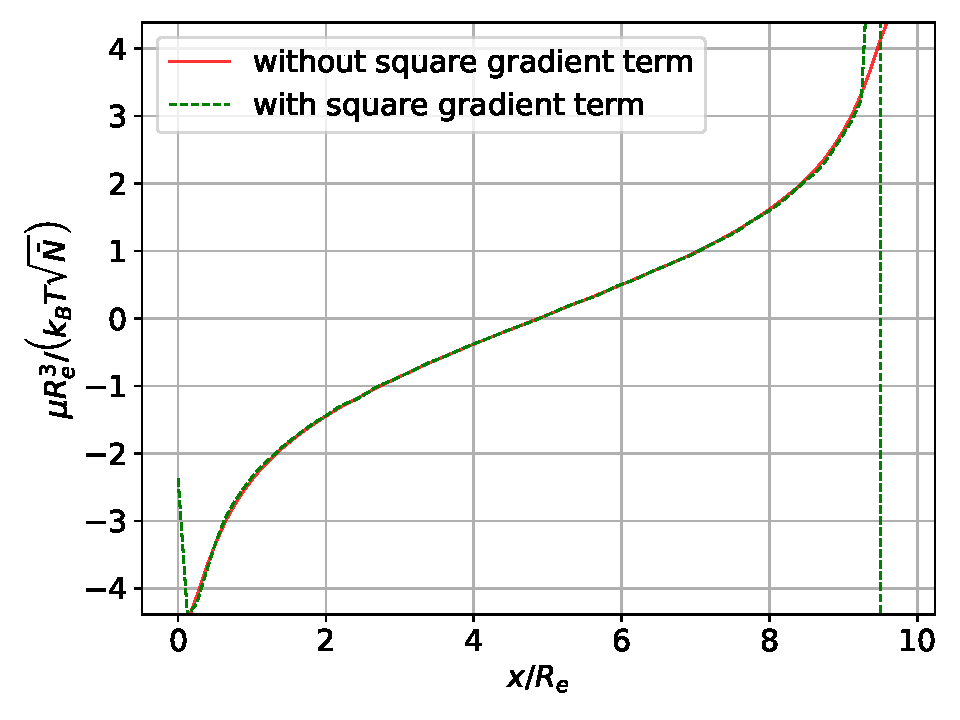
\includegraphics[width=\textwidth]{figures/mu_coll_diff.pdf}
      \caption{}
      \label{fig:chemical_potential}
  \end{subfigure}
    \hfill
  \begin{subfigure}[b]{0.45\textwidth}
      \centering
      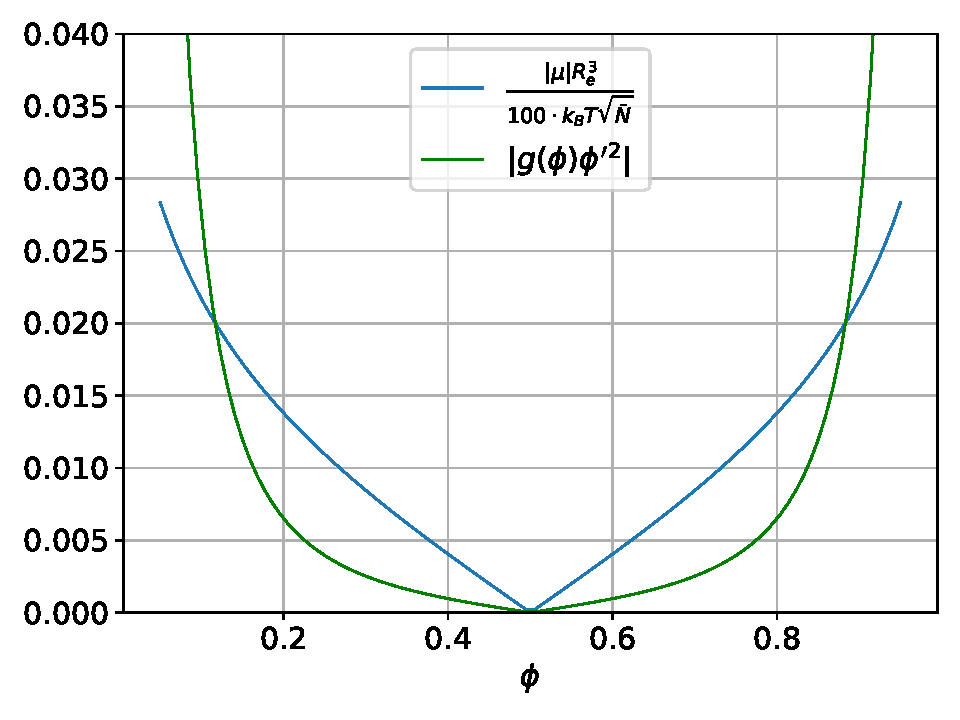
\includegraphics[width=\textwidth]{figures/squaregradient_contribution.pdf}
      \caption{}
      \label{fig:gradmu_fft}
  \end{subfigure}
     \caption{(a) Steady-state chemical potential profile obtained from \autoref{eq:mu_flory} for $r=1.0\,,$ averaged over $y$ and $z\,.$ (b) $g(\phi)\phi'^2\equiv R_e^2(1-2\phi)\phi'^2/[36\phi^2(1-\phi)^2]$ and absolute value of chemical potential $|\mu|R_e^3/(100\cdot k_BT\sqrt{\bar{N}})\,.$ In the discussed case, $\phi'\approx 0.1\,.$ }
     \label{fig:squaregradient_contribution}
\end{figure}


Evidently, the contribution of the terms involving spatial derivatives of the density to the total chemical potential is negligible, except in a very small region close to the walls. The linearity of the density profile already implies $\phi''=0$ and \autoref{fig:squaregradient_contribution} shows that the term proportional to $\phi'^2$ accounts for less than one percent of the total chemical potential for $0.12\lesssim\phi\lesssim 0.88\,,$ which roughly corresponds to the region in \autoref{fig:density_profile} that is assumed to be unaffected by boundary effects. In the subsequent discussion, the terms in \autoref{eq:mu_flory} containing spatial derivatives of $\phi$ will be neglected. This approximation improves further as the simulation box becomes infinitely long and $\phi'\rightarrow 0\,.$ However, for more complex density profiles, the contribution is of course not negligible. The gradient of the chemical potential becomes:

\begin{align}
    \frac{\nabla\mu R_e^3}{\sqrt{\bar N}k_BT}=\frac{\phi'}{\phi(1-\phi)}\,.
    \label{eq:gradmu}
\end{align}

With Equations \eqref{eq:current_local} and \eqref{eq:mu_flory}, neglecting the terms arising from the square gradient, the current calculates to:


\begin{align}
  J=-D\sqrt{\bar N}R_e^{-3}\phi'\,,
  \label{eq:current_a}
\end{align}


If the current of the normalized density is considered instead, \autoref{eq:current_a} must be devided by $\sqrt{\bar N}R_e^{-3}\,.$ Together with \autoref{eq:conti}, this gives the standard diffusion equation:
\begin{align}
  \frac{\partial\phi(\mathbf r, t)}{\partial t}-D \phi''=0\,.
  \label{eq:diffusion}
\end{align}

where $D$ is obtained from \autoref{eq:einstein_relation}. In the steady state, this simply yields $\phi''=0\,,$ so a linear density profile is obtained, as expected. From \autoref{eq:current_a}, and the condition that $\phi(L_x/2)=1/2\,,$ which follows from the symmetry of the conversion rates, the density profile becomes:

\begin{align}
  \phi(x)=\frac{JR_e^3}{D\sqrt{\bar{N}}}\left(\frac{L_x}{2}-x\right) + \frac{1}{2}\,,
  \label{eq:density_profile_ana}
\end{align}


To verify \autoref{eq:onsager}, the Onsager coefficient may also be obtained directly from the simulation results using \autoref{eq:current_local}. Again assuming local coupling and making use of \autoref{eq:gradmu}, one obtains:

\begin{align}
  \Lambda=-\frac{JR_e^3}{\sqrt{\bar N}\phi'}\phi(1-\phi).
  \label{eq:onsager_num}
\end{align}

The resulting Onsager coefficient is plotted in \autoref{fig:onsager_coeff}.

\begin{figure}[h]
  \centering
  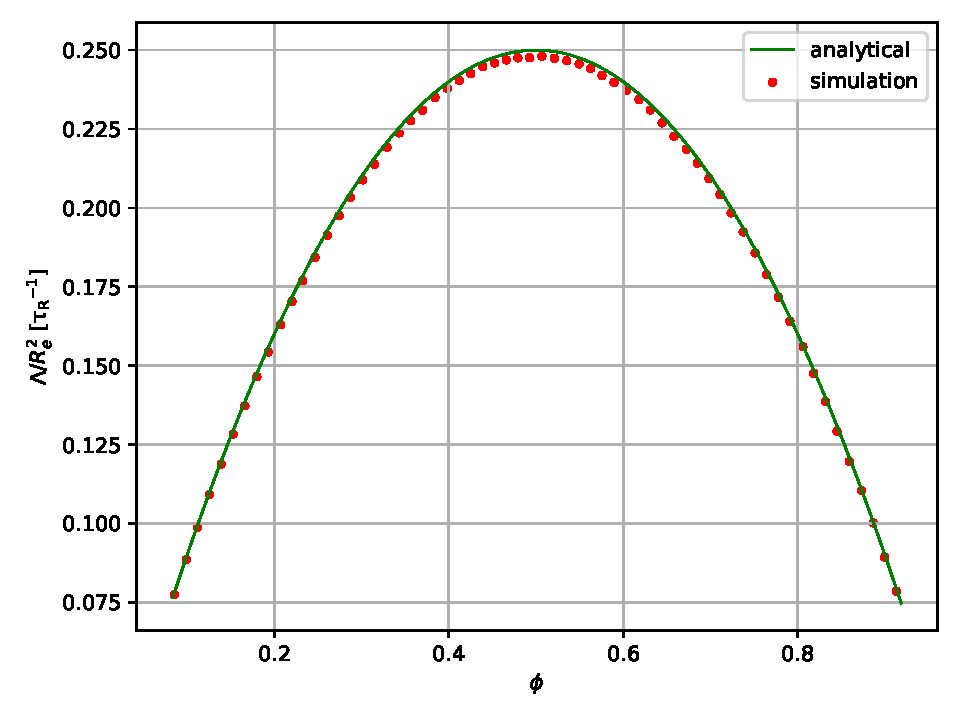
\includegraphics[width=0.6\linewidth]{figures/onsager_coll_diff.pdf}
  \caption{Onsager coefficient $\Lambda$ as a function of $\phi$. The analytical curve is obtained from Equations \eqref{eq:onsager} and \eqref{eq:density_profile_ana}, the numerical curve from \autoref{eq:onsager_num} and the density profile in \autoref{fig:density_profile}, where $\phi'$ is obtained from a linear fit. Only data points measured at a distance greater than $R_e$ from the walls are used. The diffusion constant $D$ and the current $J$ are both obtained from the simulation.}
  \label{fig:onsager_coeff}
\end{figure}

The Onsager coefficients obtained from Equations \eqref{eq:onsager} and \eqref{eq:onsager_num} are in excellent agreement, which hints that the theoretical derivations are consistent with the simulation results. 
Specifically, the assumptions of incompressibility and local coupling of the current to the chemical potential are justified and the linear density profile observed in \autoref{fig:density_profile} is explained.


\chapter{External-field-driven flow}

One of the simplest ways to implement time-dependent boundary conditions in \ac{SOMA} is to apply time-dependent external fields that are only nonzero close to the boundaries. For this, an additional, dimensionless term $f_i(\mathbf r,t)$ is added to the instantaneous fields \autoref{eq:calc_omegafields} which quantifies the excess free energy of a bead of type $i$ in the external field in units of $k_BT\,.$ In this section, layers of lamellar diblock-copolymers are moved at constant speed $v$ perpendicular to their orientation using spatially periodic external fields close to the boundaries. In the applied \ac{MC} scheme, the friction coefficient $\zeta$ in \autoref{eq:d_rouse} is determined relative to a fixed background. In a system that moves along with the external field, this background is moving at the speed $-v\,,$ so the system is not Galilei-invariant and each monomer experiences a friction force $-\zeta v\,,$ causing the whole lamellae to bend. The convective motion due to the moving fields is opposed by the diffusive motion due to the Brownian dynamics. It is therefore useful to define a P\'eclet number \cite{peclet}:

\begin{align}
    P_e= vR_e/D\,,
\end{align}


which puts the two transport mechanisms in relation on the typical length scale $R_e\,.$ For small $P_e\approx0\,,$ the chains are able to fully relax to the undeformed shape. Beyond a critical value $P_e^*\,,$ they cannot keep up with the movement of the external field anymore, which causes the lamellae to break and reconnect to the boundaries periodically. This is shown in \autoref{fig:lamella_breaking} for $P_e=0.92\,,$ the whole process happens within about half a relaxation time. In this section, an intermediate regime of $P_e$ is investigated to obtain the bending modulus $K$ of the lamellae. 


\begin{figure}[H]
    \centering
    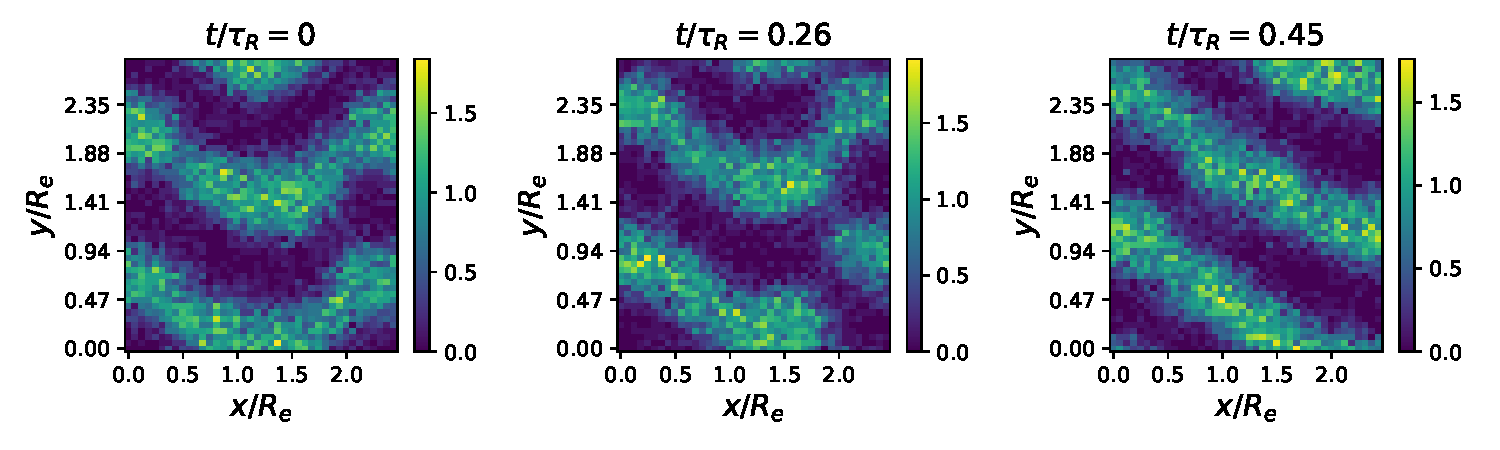
\includegraphics[width=\textwidth]{figures/lamella_breaking.pdf}
    \caption{Snapshots of the $A$ density at $P_e=0.92\,.$ Left: Shortly before breaking. Middle: Lamella breaks. Right: Broken end reconnects to nearest lamella part.}
    \label{fig:lamella_breaking}
\end{figure}


\section{Reference system}
A system of $n=750$ symmetric diblock-copolymers with and $\chi N=20$ is used. This corresponds to a lamellar phase in \autoref{fig:diblock_phasediagram}. The chain discretization is $N=32$ or $N=64\,,$ respectively. The box dimensions are $L_x\times L_y\times L_z=2.5\times2.82\times1\,R_e^3\,,$ which corresponds to $\sqrt{\bar{N}}=106\,.$ The spatial discretizations are $\Delta x=1/16\,R_e\,,$ $\Delta y=47/800\,R_e$ and $\Delta z=1\,R_e\,.$ To generate the initial lamellar structure, external fields are applied, as shown in \autoref{fig:fext}. The interlayer spacing of $\lambda=1.41\,R_e$ was found to be stable throughout the simulations, but it does not correspond to the equilibrium spacing.

Subsequently, the external fields are switched off everywhere except at a distance less than $b=0.5\,R_e$ from the boundaries in the $x$-direction, so the length of the part of the lamellae that is not supported by the external fields is $L=1.5\,R_e$. After a time $\Delta t$, the fields are moved by a distance of $\Delta y$ in the $y$-direction, so the velocity is $v=47R_e/(800\Delta t)\,.$ Snapshots of the density profile are also periodically taken after a time $\Delta t$. The external fields balance the friction forces at the boundaries and therefore act as bearings for the lamellae. The diffusion constant $D$ is obtained from \autoref{eq:einstein_relation}, where $g_3(t)$ is measured in a system without external fields and $\chi N=0\,.$

\begin{figure}[h]
    \centering
    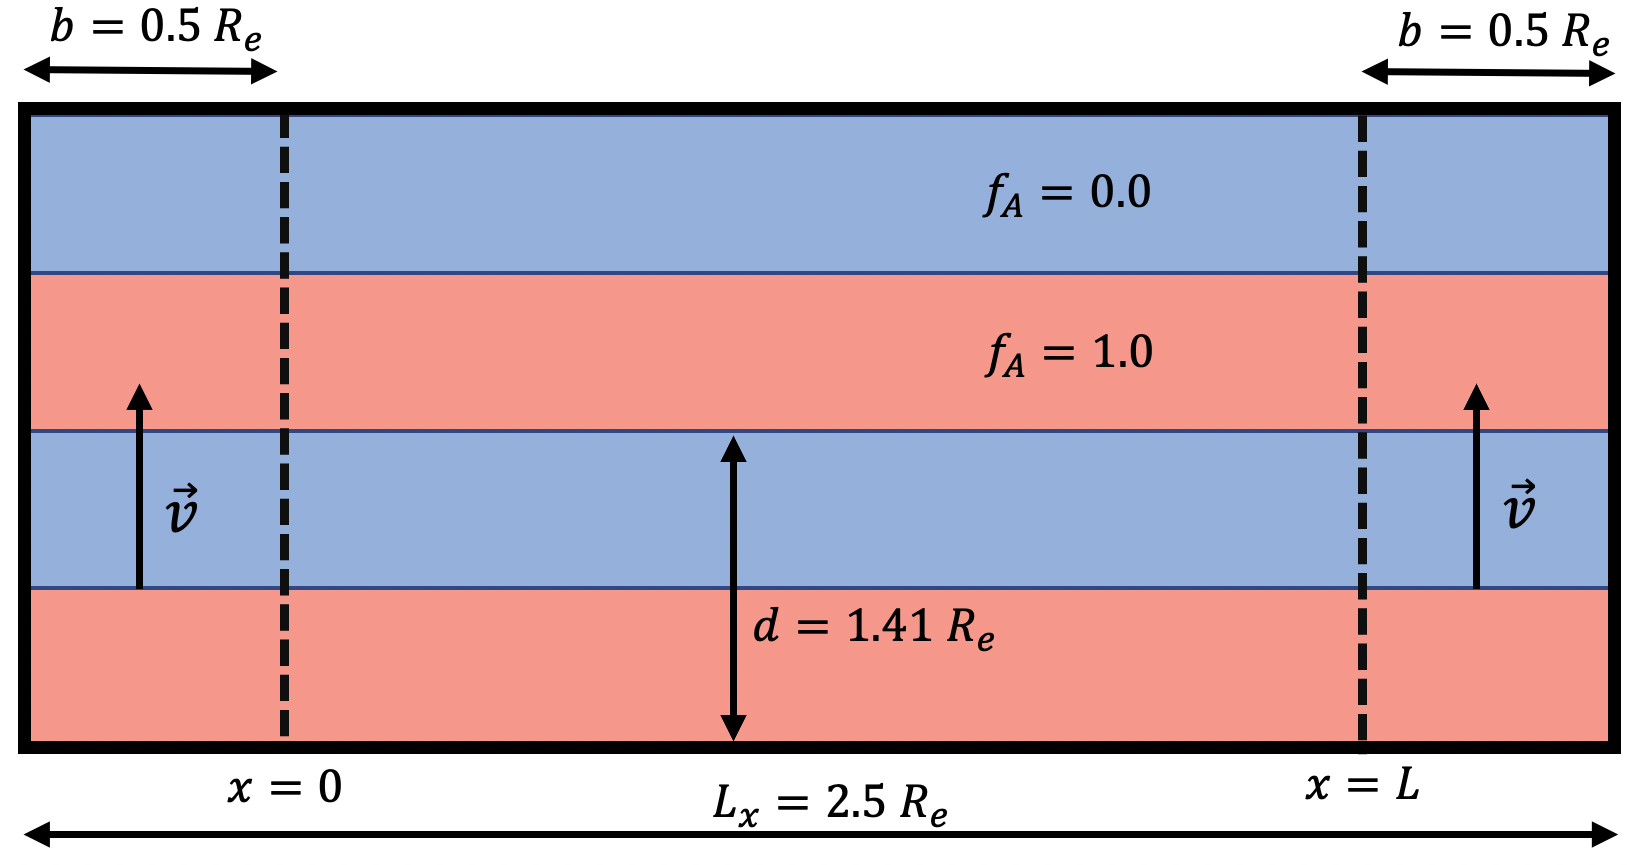
\includegraphics[width=0.6\linewidth]{figures/fext.png}
    \caption{Sketch of the external field $f_A(\mathbf r,0)\,.$ Red domains correspond to $f_A=1.0\,,$ blue domains to $f_A=0.0\,.$ $f_B(\mathbf r,0)$ is exactly complementary. Within the region bounded by the dotted lines, the external fields are switched off after the initial lamella structure has been generated.}
    \label{fig:fext}
\end{figure}


\section{Bending modulus}


Neglecting any change in the lamellar spacing, in the \ac{SSL}, the free energy of a bent lamella is \cite{wang94}:

\begin{align}
    F&=\int d\mathbf r\left\{f_0+\frac{1}{2}K \left(\partial_x^2 u\right)^2\right\}\,,\\
    &\approx \lambda L_z\int dx\left\{f_0+\frac{1}{2}K \left(\partial_x^2 u\right)^2\right\}\nonumber\\
    &\equiv \lambda L_z\int dxf(u'')\,.
    \label{eq:F_bend}
\end{align}

where $f_0$ is the free energy per unit volume of the unbent lamella, $K$ is the bending modulus and $u\equiv u(x)$ is the deformation profile of the A-B-interface. Due to the bending, the lamellae also experience a volume change which is neglected in the integration. The friction force density is $q_{fric}=\rho_0\zeta v=N\sqrt{\bar N}\zeta P_eD/R_e^4\,.$ In the steady-state, it is balanced by a force density given by the  functional derivative $\delta F/\delta u\,$:

\begin{align}
    \frac{\delta F}{\delta u}&=\frac{\partial^2}{\partial x^2}\frac{\partial f}{\partial u''}\overset{!}{=}q_{fric} \nonumber \\
    \implies K\frac{\partial^4u}{\partial x^4}&=N\sqrt{\bar N}\zeta\frac{P_eD}{R_e^4} \,.
\end{align}


With the boundary conditions $u(0)=u(L)=0$ and $u''(0)=u''(L)=0\,,$ one obtains:
\begin{align}
    u(x)=\frac{N\sqrt{\bar N}\zeta P_e D}{24KR_e^4}x(L^3-2Lx^2+x^3)\,,
    \label{eq:deflection}
\end{align}
in analogy to a beam bending under a uniform load in the Euler-Bernoulli theory. The resulting lamellar profiles are shown in \autoref{fig:deflection_N32} for $N=32\,.$ Due to the periodic boundary conditions, the zero point of the $y$ axis can be shifted arbitrarily. This is exploited such that a whole $A$-lamella can be displayed in the lower half of the coordinate system, e.g., for $y<\lambda =l_y/2\,.$ \autoref{fig:deflection_N32}a shows the average of both $A$-lamella in the system. Since the boundaries between two adjacent monolayers are not sharp, the \enquote{center of mass curve} is used instead to describe the one dimensional lamella profile. The deformation curve $u(x)$ is obtained as

\begin{align}
    u(x)=\left |\frac{1}{\hat\phi_A(x)}\left(\sum_{i=0}^{n_y/2-1}i\Delta y \hat\phi_A(x,i\Delta y)\right)-y_0\right |\,,
    \label{eq:rcm_curve}
\end{align}

where $\hat\phi_A(x)=\sum_{i=0}^{n_y/2-1}\hat\phi_A(x,i\Delta y)$ is the total $A$-density as a function of $x\,.$ $n_y=l_y/\Delta y$ is the number of grid points in the $y$ direction and $y_0$ is the center of mass of the $A$-block at $x=0\,,$ as indicated in \autoref{fig:deflection_N32}a. \autoref{eq:rcm_curve} assumes that only a single $A$-block is considered, without interference from neighboring $A$-blocks. \autoref{fig:deflection_N32}b shows the fit of \autoref{eq:rcm_curve} to \autoref{eq:deflection}. For $P_e=0.24$, the fit is in excellent agreement with the simulation data. $P_e=0.85\approx P_e^*$ was found to be the critical P\'eclet number beyond which the lamellae break. For these large deformations, the fit displays deviations from the simulation data, especially around the maximum. This error is systematic, since, for large deformations, the vertical extension of a single $A$-block is approximately $\lambda\,,$ and, therefore, $A$-blocks from the neighboring bilayer interfere with the computation of \autoref{eq:rcm_curve}. 

\begin{figure}[H]
    \centering
    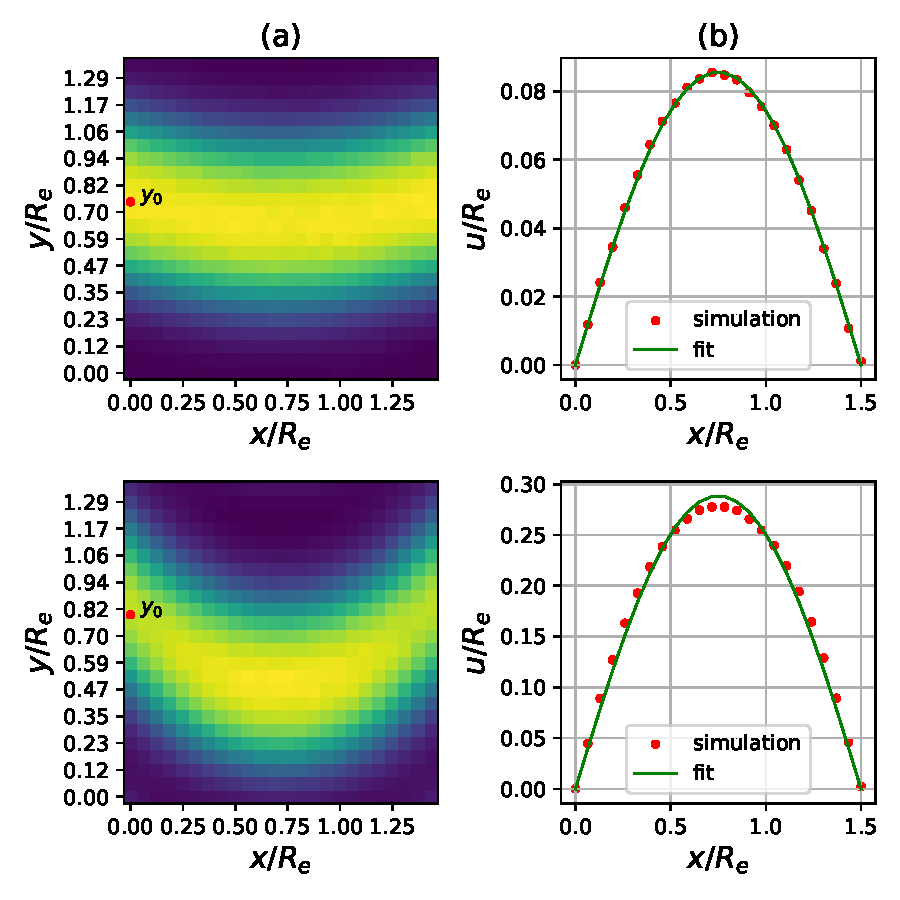
\includegraphics[width=\linewidth]{figures/deflection_N32.pdf}
    \caption{(a) Heatmap of the steady-state lamella profile in the reference frame that moves with the external field, averaged over all lamellae. (b) Lamella deformation curve obtained from \autoref{eq:rcm_curve}. The fit corresponds to \autoref{eq:deflection}. The top row corresponds to $P_e=0.24\,.$ The bottom row corresponds to $P_e=0.85\,.$}
    \label{fig:deflection_N32}
\end{figure}



The maximum deformation is:
\begin{align}
    u_{max}=u(L/2)=\frac{5N\sqrt{\bar N}\zeta P_e DL^4}{384KR_e^4}\,.
    \label{eq:umax}
\end{align}

To obtain the bending modulus, $u_{max}$ is measured for various values of $P_e\,$, this is shown in \autoref{fig:stress_strain}. Values corresponding to $P_e>0.7$ are discarded due to the systematic error for large deformations. Figure \autoref{fig:K_N} shows that the bending modulus is proportional to $1/N\,.$




\begin{figure}[h]
  \centering
 \begin{subfigure}[b]{0.45\textwidth}
    \centering
    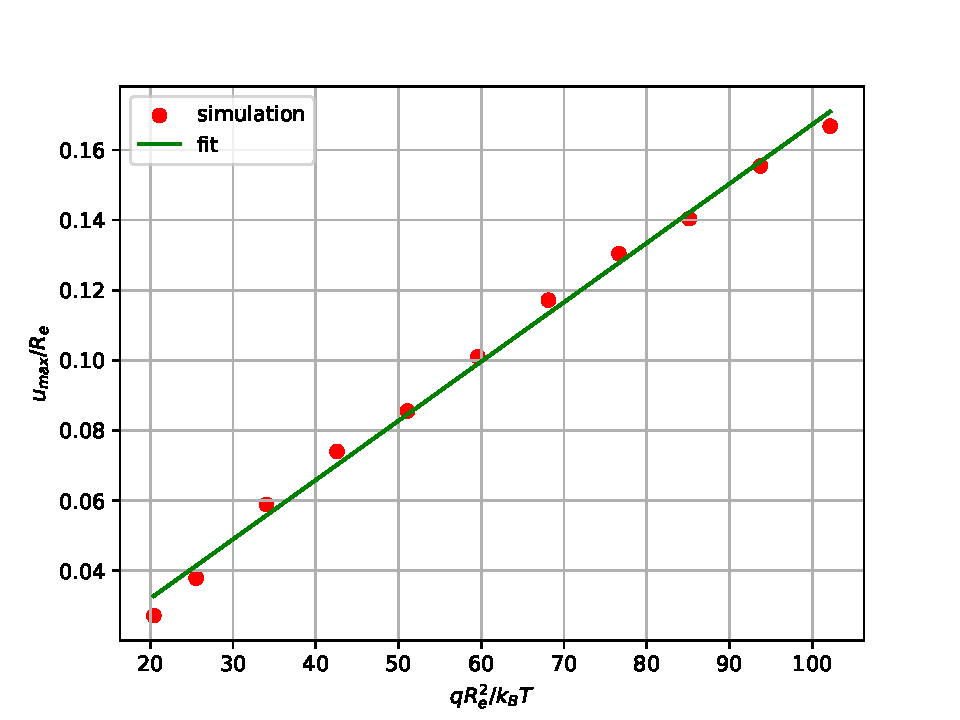
\includegraphics[width=\textwidth]{figures/stress_strain_plot.pdf}
    \caption{}
    \label{fig:stress_strain}
\end{subfigure}
    \hfill
  \begin{subfigure}[b]{0.45\textwidth}
      \centering
      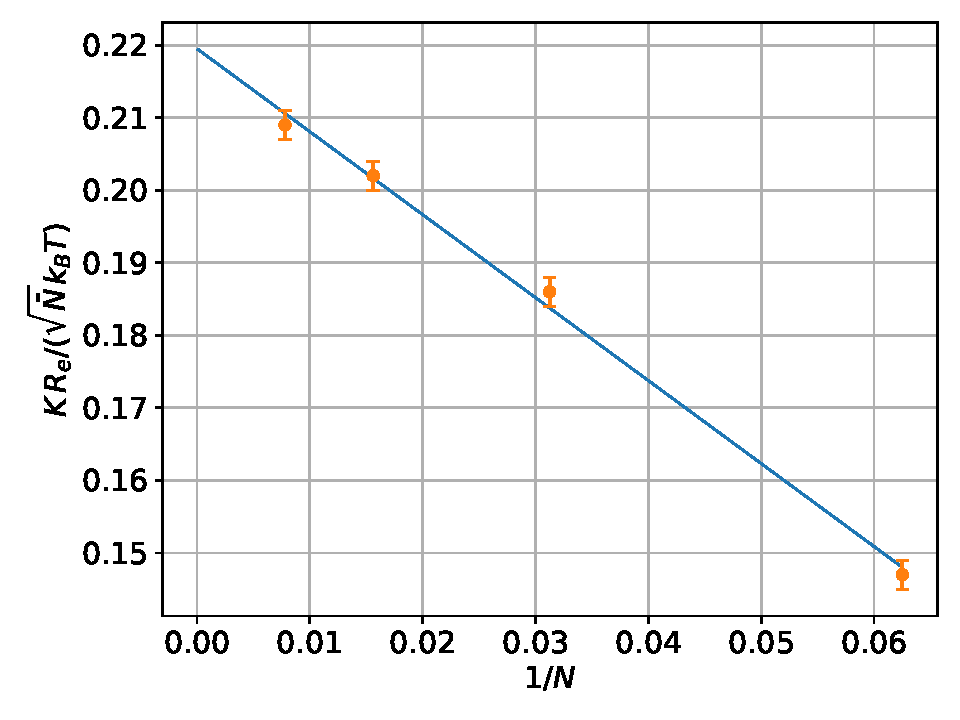
\includegraphics[width=\textwidth]{figures/K-N.pdf}
      \caption{}
      \label{fig:K_N}
  \end{subfigure}
     \caption{(a) Maximum deformation $u_{max}$ as a function of the P\'eclet number $P_e\,.$ The fits correspond to \autoref{eq:umax}. (b) Bending modulus $K$ plotted over $1/N\,.$}
\end{figure}


Alternatively, $K$ may also be obtained from \ac{SCFT}. While a detailed discussion of \ac{SCFT} is omitted in this thesis, it should be mentioned that, unlike in the particle-based \ac{SCMF} simulations, the chains are treated as continuous density fields with $N\rightarrow \infty\,.$ The system is forced away from equilibrium by constraining the $A$-$B$-interface to a sinusoidal deformation $u(x)=a\sin 2\pi x/L\,,$ as shown in the inset of \autoref{fig:bend_scft}. From \autoref{eq:F_bend}, the total free energy may be calculated as:

\begin{align}
    F&\approx\lambda L_z\int dx\left\{f_0+\frac{1}{2}Ka^2\left(\frac{2\pi}{L}\right)^4\sin\left(\frac{2\pi}{L}x\right)^2\right\}\nonumber\\
    &= \lambda LL_zf_0+\lambda L_z\frac{4\pi^4a^2}{L^3}K\,.
    \label{eq:f_scft_1}
\end{align}

On the other hand, the total free energy may be obtained by integrating the free energy density over the lamella volume:
\begin{align}
    F&=\int d\mathbf r(f_0+f_b)\nonumber\\
    &\approx \lambda LL_z(f_0+f_b)\nonumber \\
    &=\lambda LL_z\frac{\sqrt{\bar N}}{R_e^3}(\tilde f_0+\tilde f_b)\,,
    \label{eq:f_scft_2}
\end{align}

where $\tilde f_0=4.0337\,k_BT$ is the free energy per chain of the undeformed lamella and $\tilde f_b=0.79278\,k_BT(a/R_e)^2$ is the free energy per chain due to the deformation. Comparing Equations \eqref{eq:f_scft_1} and \eqref{eq:f_scft_2}, the bending modulus reads:

\begin{align}
    K_\text{SCFT}=\frac{\tilde f_b\sqrt{\bar N}}{4a^2\pi^4}R_e^{-3}L^4\,.
\end{align}

The result is $K_\text{SCFT}=0.16\,\sqrt{\bar N}k_BT/R_e\,.$ Extrapolation from the linear fit in \autoref{fig:K_N} to $N\rightarrow\infty$ gives $K_\infty=0.22\,\sqrt{\bar N}k_BT/R_e\,.$ Furthermore, the difference may arise from the different mechanisms that are used to keep the systems away from equilibrium: the moving external field in the \ac{SCMF} simulation and the interfacial constraint in the \ac{SCFT} simulations.

% \begin{itemize}
%     \item The following discussion can probably be omitted
% \end{itemize}

% In equilibrium, it may also be obtained directly from the simulation parameters \cite{wang94}:


% \begin{align}
%     K=\frac{3}{16}\left(\frac{12}{\pi^2}\right)^{1/3}\left(\frac{\gamma}{k_BT}\right)^{4/3}\bar N^{-1/6}R_e^{5/3}k_BT\,,
%     \label{eq:k_ana}
% \end{align}

% where $\gamma$ is the interfacial tension. In the strong segregation limit, it reads (\textbf{Hier evtl Faktor 3 wegen 3 Grenzflaechen?})\cite{semenov1996}:

% \begin{align}
%     \frac{\gamma R_e^2}{\sqrt{\bar N}k_BT}=\sqrt{\frac{\chi N}{6}}\left(1-\frac{4\ln 2}{\chi N}\right)\,.
% \end{align}


% The result is $K=38.94\,k_BT/R_e\,,$ in excellent agreement with the simulation results. However, it should be noted that $\autoref{eq:k_ana}$ is derived from the equilibrium spacing $d_0\,.$ For $\chi N=20\,,$ \cite{wang94} predicts $d_0=1.24\,R_e\,,$ which is too small (\textbf{Need some reference value here to cite}). This is likely to indicate that the strong segregation is not fully reached at $\chi N=20\,.$ Nevertheless, the results might suggest that the bending modulus $K$ only weakly depends on the monolayer tickness.


\begin{figure}[H]
    \centering
    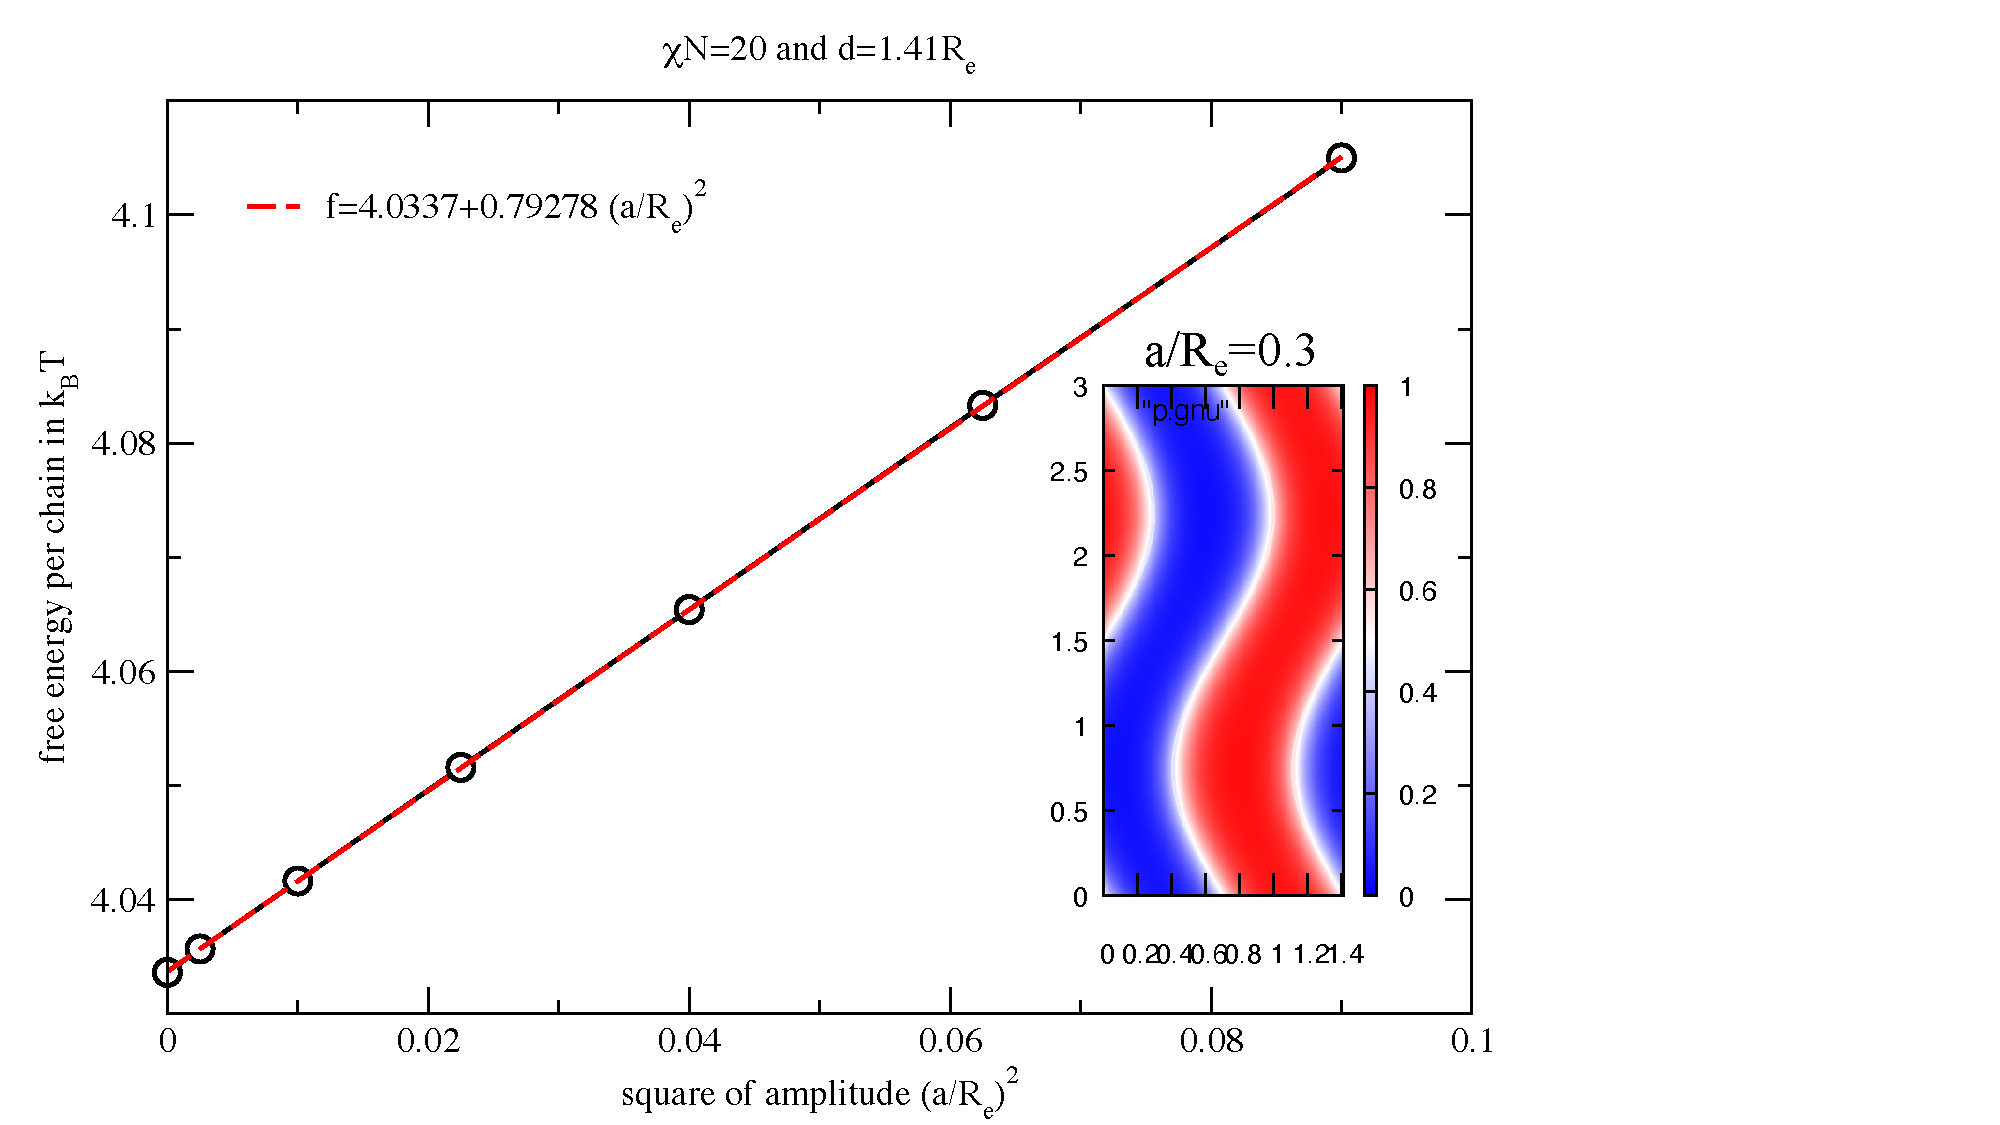
\includegraphics[width=0.6\linewidth]{figures/bend_scft.pdf}
    \caption{Free energy per chain as a function of the square of the amplitude from exact \ac{SCFT} calculations. The inset shows the lamella cross-section for $a/R_e=0.3\,.$}
    \label{fig:bend_scft}
\end{figure}


\chapter{Polymer-type-conversion-based target composition}
\label{chap:polyconversion}

\section{Formulation of the problem}
We now want to take a step towards simulating the setting depicted in \autoref{fig:continuum_section}. If one considers two opposing sides from the rectangular section cut out of the larger continuum simulation, then the time-evolution of the density will, in general, be completely different on both walls. Therefore, periodic boundary conditions cannot be applied. Instead, the simulation box is bounded by hard, impenetrable walls in \ac{SOMA}. As discussed previously, the proximity area of these walls is entropically disfavored, leading to a decrease in the total density. This is problematic, since it is exactly this region where one wishes to dictate a target composition. Another issue is caused by the fluctuation of the total density, which is one of the key features of \ac{SCMF} simulations. A way out is to dictate the composition instead:

\begin{align}
    \tilde\phi_\alpha(c)=\frac{\hat\phi_\alpha(c)}{\sum_{i=1}^{n_t}\hat\phi_i(c)}\,.
\end{align}

It brings the advantage that the compositions of different types always sums to one. However, it is undefined for empty cells, so these must be ignored. To dictate the composition in specific cells, target values $\tilde\phi_{\alpha,T}(c)$ are defined, with $\tilde\phi_{\alpha,T}(c)=-1\forall\alpha\,,$ a purposefully unphysical value, for cells in which no target composition is desired. In the following, the cells $c$ for which $\tilde\phi_{\alpha,T}(c)\ge 0$ $\forall\alpha$ are called \enquote{target cells}. Mixed cells with $\tilde\phi_{\alpha,T}(c)\ge 0$ for some $\alpha$ and $\tilde\phi_{\alpha,T}(c)<0$ for other $\alpha$ are not allowed and target cells must fulfill the condition $\sum_\alpha\tilde\phi_{\alpha,T}(c)=1\, .$ The total number of target cells is denoted $n_T\,.$ Let $n_p$ be the number of polymers that have at least one monomer in any target cell $c\,.$ In the following, these polymers are called \enquote{target polymers}. Instead of using external fields, like in the previous section, the goal is to reach the target composition by switching polymer types, see \autoref{chap:colldiff}. In this thesis, only conversions between macromolecule types with the same bond topology are considered. Due to the chain connectivity, this leads to a complex optimization problem, which aims to minimize the following loss function:

\begin{align}
    L[\{\hat\phi_i\}]=\sum_{\alpha=0}^{n_t}\sum_{c\in \{\text{cells}\}}\theta(\tilde\phi_{\alpha,T}(c))\left(\tilde\phi_\alpha(c)-\tilde\phi_{\alpha,T}(c)\right)^2\,,
    \label{eq:lossfunction}
\end{align}

where $\theta(\tilde\phi_{\alpha,T}(c))=1$ if $\tilde\phi_{\alpha,T}(c)\ge 0$ and $\theta(\tilde\phi_{\alpha,T}(c))=0$ otherwise. Since the compositions $\tilde\phi_\alpha(c)$ depend on the target polymer types, the search space $\Omega$ consists of all possible combinations of target polymer types. To minimize \autoref{eq:lossfunction}, one must first define the notion of a neighboring solution. If $\pmb{\beta}=\{\beta_1,\dots,\beta_j,\dots\beta_{n_p}\}\in\Omega$ is the current configuration of polymer types, then we define a neighboring solution as $\pmb{\beta}^*=\{\beta_1,\dots,\beta^*_j,\dots\beta_{n_p}\}\in\Omega\,,$ where the type of the $j$th target polymer is changed from $\beta_j$ to $\beta_j^*$ and every other polymer type is unchanged. In the following, this rule to generate a neighboring solution is called a \enquote{flip}. \autoref{eq:lossfunction}, together with the flip rule, defines a non-convex discrete optimization problem. The non-convexity can easily be seen by looking at the simple example for $n=4$ homopolymers with $N=2$ on a $2\times 2$ grid shown in \autoref{fig:loss}.


\begin{figure}[H]
  \centering
  \begin{subfigure}[b]{0.25\textwidth}
      \centering
      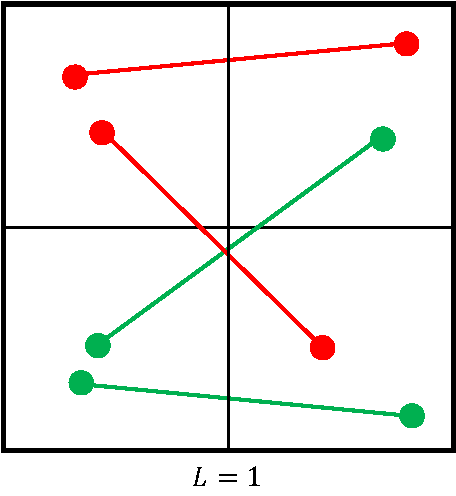
\includegraphics[width=\textwidth]{figures/loss-1.pdf}
      \caption{}
      \label{fig:loss-1}
  \end{subfigure}
    \hfill
  \begin{subfigure}[b]{0.25\textwidth}
      \centering
      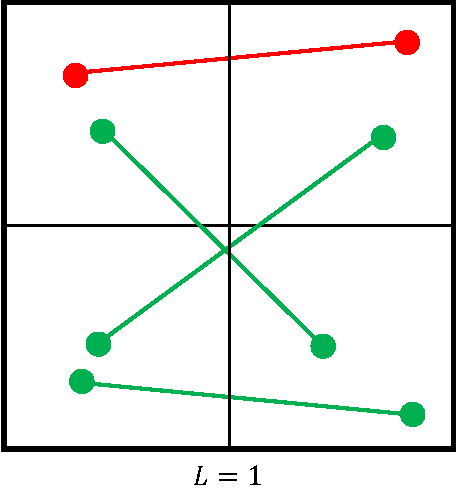
\includegraphics[width=\textwidth]{figures/loss-2.pdf}
      \caption{}
      \label{fig:loss-2}
  \end{subfigure}
      \hfill
  \begin{subfigure}[b]{0.25\textwidth}
      \centering
      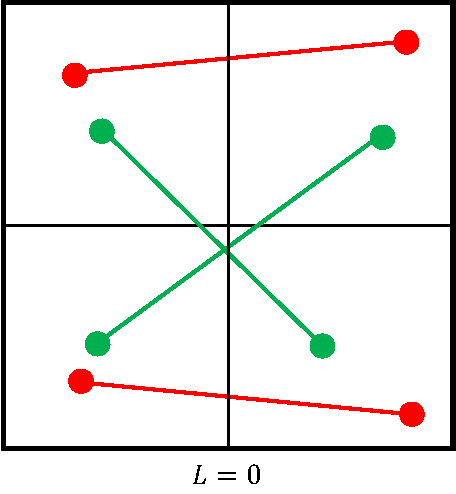
\includegraphics[width=\textwidth]{figures/loss-3.pdf}
      \caption{}
      \label{fig:loss-3}
  \end{subfigure}
     \caption{Example for $n=4$ homopolymers with $N=2$ on a $2\times 2$ grid to show that the loss function defined by \autoref{eq:lossfunction} is, in general, non-convex under the type-switch of a single polymer. The target compositions are $\tilde\phi_{A,T}=\tilde\phi_{B,T}=0.5$ for all cells.}
     \label{fig:loss}
\end{figure}

In \autoref{fig:loss-1}, any possible flip will not decrease the value of $L\,.$ \autoref{fig:loss-2} shows the configuration after conversion of a red polymer to a green one. A flip of the polymer at the bottom now decreases the loss function, as shown in \autoref{fig:loss-3}. It should be noted that this minimum is not unique, since a flip of every polymer would also yield $L=0\,.$

The target polymers are identified and saved to a list by \autoref{alg:get_flip_candidates}.

\begin{algorithm}[H]
\caption{Get target polymers}\label{alg:get_flip_candidates}
\begin{algorithmic}[1]
\State Let $polyIsTarget[n]$ be a new boolean array initialised with $0$'s
\State $n_p\gets 0$
\For{$poly\gets 0$ to $n-1$}
    \For{$monomer\gets 0$ to $N-1$}
        \State $monoCell\gets$\textit{cell index of monomer}
        \If{target composition available for $monoCell$}
            \State $polyIsTarget[poly]\gets 1$
            \State $n_p\gets n_p+1$
            \State \textbf{break}
        \EndIf
    \EndFor
\EndFor
\State Let $targetPolyIndices[n_p]$ be a new array
\State $i\gets 0$
\For{$poly\gets 0$ to $n-1$}
\Comment{Store indices of target polymer to new array}
    \If{$polyIsTarget[poly]==1$}
        \State $targetPolyIndices[j]\gets poly$
        \State $j\gets j+1$
    \EndIf
\EndFor
\end{algorithmic}
\end{algorithm}
 
A boolean array of length $n$ is declared and all values are set to zero. An iteration over all polymers and the corresponding monomers is performed. The monomers are assigned to a cell and it is checked if a target composition is available for that cell. If so, the corresponding entry for the polymer in the boolean array is set to one and the next polymer is considered. The number of target polymers $n_p$ is also determined in this process. For a quicker access to the target polymers, their indices are stored sequentially in a separate array of length $n_p\,.$ This requires dynamic memory allocation since $n_p$ varies during the simulation and it cannot be determined analytically. The cell index of the $k$th target cell in which a target polymer $j$ has monomers is saved to an $n_p\times N$ matrix $\tilde q$ with entries $\tilde q_{jk}\,.$ The number of target cells over which a target polymer $j$ extends is denoted $n_{cells,j}\,.$ It is not actually used in the implementation, however, it simplifies the discussion. $n_{cells,j}$ may take any integer value between $1$ and $N\,,$ this is incorporated by setting $\tilde q_{jk}<0$ for $k\ge n_{cells,j}\,.$ Let $\tilde n$ be the $n_p\times m_t\times n_t\times N$ matrix with entries $\tilde n_{j\beta\alpha k}$ that holds the number of monomers of type $\alpha$ that target polymer $j$ has in the $k$th target cell if it has the molecule type $\beta\,,$ where $\tilde n_{j\beta\alpha k}=0$ for $k\ge n_{cells,j}\,.$ An example is shown in \autoref{fig:cell_info} for a binary mixture of homopolymers with $n_p=2\,,$ $N=8$ and $n_T=6\,.$


\begin{figure}[h]
    \centering
    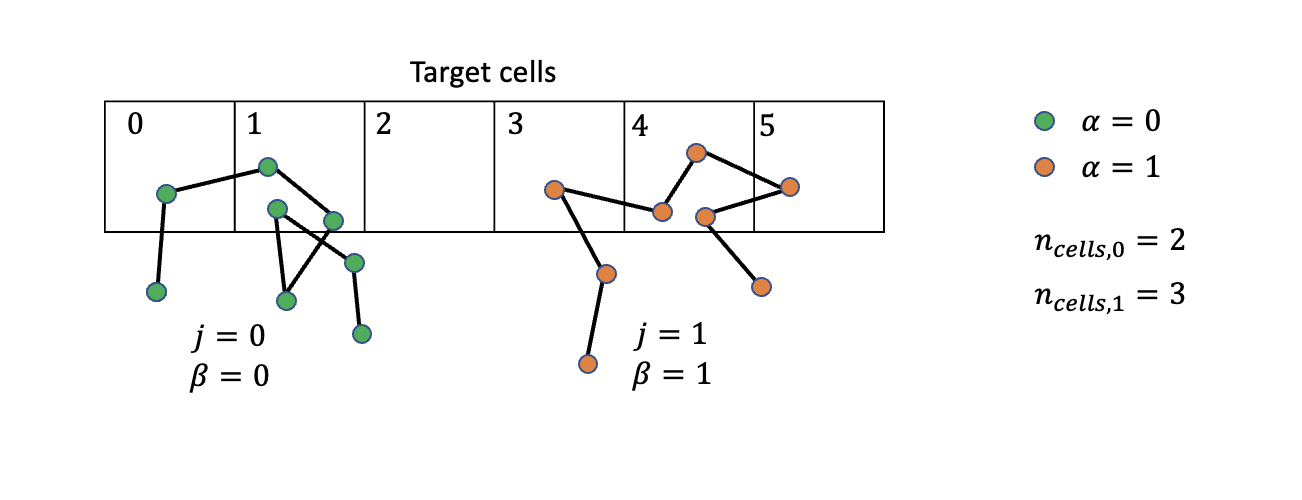
\includegraphics[width=
    \linewidth]{figures/cell_info.png}
    \caption{Example to explain the setting discussed in the text. $\beta$ denotes the polymer type and $\alpha$ denotes the monomer type. For homopolymers, distinguishing between the two is redundant. For demonstration purposes, the differentiation is still made here.}
    \label{fig:cell_info}
\end{figure}

The example corresponds to

\begin{align*}
    \tilde q=
    \begin{bmatrix}
    0 & 1 & -1 & -1 & -1 & -1 \\
    3 & 4 & 5 & -1 & -1 & -1 \\
    \end{bmatrix}
\end{align*}

and the only non-zero submatrices

\begin{align*}
    \tilde n_{j00k}=\tilde n_{j11k}
    \begin{bmatrix}
    1 & 3 & 0 & 0 & 0 & 0 \\
    1 & 3 & 1 & 0 & 0& 0 \\
    \end{bmatrix}\,.
\end{align*}

of $\tilde n\,.$ Any submatrices corresponding to $\alpha\neq\beta$ only have zero-entries since homopolymers are considered.

After the flip $\beta_j\rightarrow \beta_j^*$ of an arbitrary target polymer $j\,,$ the value of the loss function is updated according to:

\begin{align}
    L^*_{\beta_j\rightarrow\beta_j^*}[\{\hat\phi_i\}] &= L[\{\hat\phi_i\}] 
    - \sum_{\alpha=0}^{n_t}\sum_{k=0}^{n_{cells,j}-1}  \left(\hat\phi_\alpha(\tilde q_{jk})-\tilde\phi_{\alpha,T}(\tilde q_{jk})\right)^2\nonumber \\
    & \quad + \sum_{\alpha=0}^{n_t}\sum_{k=0}^{n_{cells,j}-1}  \left(\hat\phi_\alpha(\tilde q_{jk})+\Delta\hat\phi_{ j\alpha k}(\beta\rightarrow\beta^*)-\tilde\phi_{\alpha,T}(\tilde q_{jk})\right)^2\nonumber \\
    &= L[\{\hat\phi_i\}] 
    + \sum_{\alpha=0}^{n_t}\sum_{k=0}^{n_{cells,j}-1}  \biggl\{\Delta\hat\phi^2_{ j\alpha k}(\beta\rightarrow\beta^*) \nonumber\\
    &\quad + 2\Delta\hat\phi_{ j\alpha k}(\beta\rightarrow\beta^*)\left(\hat\phi_{\alpha}(\tilde q_{jk})-\tilde\phi_{\alpha,T}(\tilde q_{jk})\right)\biggr\}
\end{align}

where $\Delta\hat\phi_{ j\alpha k}(\beta_j\rightarrow\beta_j^*)\equiv\tilde n_{j\beta_j^*\alpha k}-\tilde n_{j\beta_j\alpha k}$ is the change in the density of type $\alpha$ in cell $\tilde q_{jk}$ due to the flip $\beta_j\rightarrow\beta_j^*\,$. Thus, for an efficient implementation of an optimization algorithm, the matrices $\tilde q$ and $\tilde n$ have to be determined first. For the determination of the unique target cells of a given target polymer, one first has to iterate again over all its bead positions and determine the corresponding cells using the assignment function in \autoref{eq:normalized_densities}. The cells are then sorted by their indices and the unique ones are identified. This is described in \autoref{alg:get_cell_indices}. 


\begin{algorithm}[H]
\caption{Get unique target cells}\label{alg:get_cell_indices}
\begin{algorithmic}[1]
\State Let $targetPolyCells[n_p][N]$ be a new array initialised with $-1$'s
\For{$i\gets 0$ to $n_p-1$}
\Comment{Loop over target polymer}
    \State $poly \gets polymers[targetPolyIndices[i]]$
    \State let $monoCells[N]$ be a new array
    \State $j\gets 0$
    \For{$monomer\gets 0$ to $N-1$}
    \Comment{Store all target cells to monoCells}
        \State $monoCell\gets$\textit{cell index of monomer}
        \If{Target composition available for $monoCell$}
            \State $monoCells[j]\gets monoCell$
            \State $j\gets j+1$
            \State \textbf{break}
        \EndIf
    \EndFor
    \State quicksort($monoCells\,,0\,,j-1$)
    \State $k\gets 0$
    \For{$monomer\gets 0$ to $j-1$}
    \Comment{Find unique cells}
        \If{$monoCells[monomer]\neq monoCells[monomer+1]$}
            \State $targetPolyCells[i][k]\gets monoCells[monomer]$
            \State $k\gets k+1$
        \EndIf
    \EndFor
    \State $targetPolyCells[i][k]\gets monoCells[j-1]$
\EndFor
\end{algorithmic}
\end{algorithm}

This may seem tedious, however, it is necessary since a polymer can leave a given cell and reenter it at later segments, see \autoref{fig:cell_info}. For a homopolymer, the number of monomers it has of type $\alpha$ in a target cell $c$ is simply given by the polymer type and the number of monomers it has in that cell. For a copolymer, it is necessary to compute the exact number of monomers it has of a given type in a given target cell, for each possible architecture it can assume. How this is done in \ac{SOMA} is explained in \autoref{alg:get_cell_numbers}. The algorithm assumes that the matrix $\tilde q$ has already been calculated. 

\begin{algorithm}[H]
\caption{Get monomer numbers}\label{alg:get_cell_numbers}
\begin{algorithmic}[1]
\State Let $polyCellNum[n_p][m_t][n_t][N]$ be a new array initialized with $0$'s
\For{$i\gets 0$ to $n_p-1$}
\Comment{Loop over target polymer}
    \State $poly \gets polymers[targetPolyIndices[i]]$
    \State $initialPolytype\gets poly.type$
    \For{$polyType\gets 0$ to $m_t-1$}
        \State $poly.type\gets polyType$
        \Comment Temporarily change polymer type
        \For{$monomer\gets 0$ to $N-1$}
            \State $monoCell\gets$ \textit{cell index of monomer}
            \State $monoType\gets$ \textit{bead type of monomer}
            \For{$j\gets 0$ to $N-1$}
            \Comment{Find corresponding entry}
            \If{$targetPolyCells[i][j]==monoCell$}
                \State Increment $polyCellNum[i][polyType][monoType][j]$ by 1 
                \State \textbf{break}
            \EndIf
            \EndFor
        \EndFor
    \EndFor
    
    \State $poly.type\gets initialPolytype$
    \Comment Restore polymer type
\EndFor
\end{algorithmic}
\end{algorithm}



\section{Steepest Descent}

In the \ac{SD} algorithm, which is a greedy algorithm, target polymers are selected at random and flipped to a random target type. If a flip decreases the loss function, it is accepted. Otherwise, it is rejected and the type of the according target polymer is reset to the previous type. This process is repeated until no more flips are accepted, out of $n_p$ trials. Subsequently, one more flip trial is performed for each target polymer. This algorithm will get stuck in the first local minimum that it reaches.

\section{Simulated annealing}

To avoid becoming trapped in local minima, the \ac{SA} algorithm described in \autoref{sec:sa} is employed. On average, the algorithm attempts to flip each target polymer once at each temperature. The implementation is shown in \autoref{alg:sa}. The \ac{SD} algorithm is run on the final configuration to ensure that at least a local minimum of \autoref{eq:lossfunction} is reached.

\begin{algorithm}[H]
\caption{Simulated annealing}\label{alg:sa}
\begin{algorithmic}[1]
\State $S \gets$ current configuration of target polymer types
\State $S_\text{best}\gets S$
\State $T \gets T_0$
\While{$T>T_f$}
    \State $n_{flip} \gets 0$
    \While{$n_{flip}<n_{max}$}
        \State generate new configuration $S^*$ by flipping a random polymer
        \State $n_{flip}\gets n_{flip}+1$
        \State $\Delta L\gets L(S^*)-L(S)$
        \State $r\gets$ random number between 0 and 1
        \If{$r<\exp(-\frac{\Delta L}{T})$}
            \State $S\gets S^*$
        \EndIf
    \EndWhile
\If{$L(S)<L(S_\text{best})$}
    \State $S_\text{best}\gets S$ \Comment{Update best solution}
\EndIf
\State $T\gets T-\alpha$ \Comment{or different cooling schedule}
\EndWhile
\end{algorithmic}
\end{algorithm}

\section{Comparison of algorithms}


In order to compare the performance of the two presented algorithms, several randomly generated initial configurations are optimized with lamellar target compositions. A binary blend of homopolymers with $N=32$ and $\sqrt{\bar N}=100$ is used. The box dimensions are $L_x\times L_y\times L_z=5\times5\times5\,R_e^3$ with $\Delta L=1/8\,R_e$ and hard, impenetrable walls are applied at all boundaries. The target composition is defined directly behind the walls with a width of one grid point. The lamellar target structure is a piecewise constant function that depends only on $x$ and is characterized by the periodicity $\lambda$ and the target deviation $\Delta\tilde\phi$ from the composition of the homogeneous value $0.5\,.$  The optimized structure obtained using the \ac{SD} algorithm is shown in \autoref{fig:conversion_box} for $\lambda=2\,R_e$ and $\Delta\tilde\phi=0.5\,.$ The loss function is normalized by the number of monomer types $n_t$ and the number of target cells $n_T$ to obtain the mean squared deviation from the target composition. The thermal density variance $\sigma_0^2$ is taken as a reference value. It is calculated as $\sigma_0^2=1/\rho_0\Delta L^3\kappa$ in the mean field approximation \cite{Daoulas06}. Two different cooling schedules are investigated.


\begin{figure}[h]
    \centering
    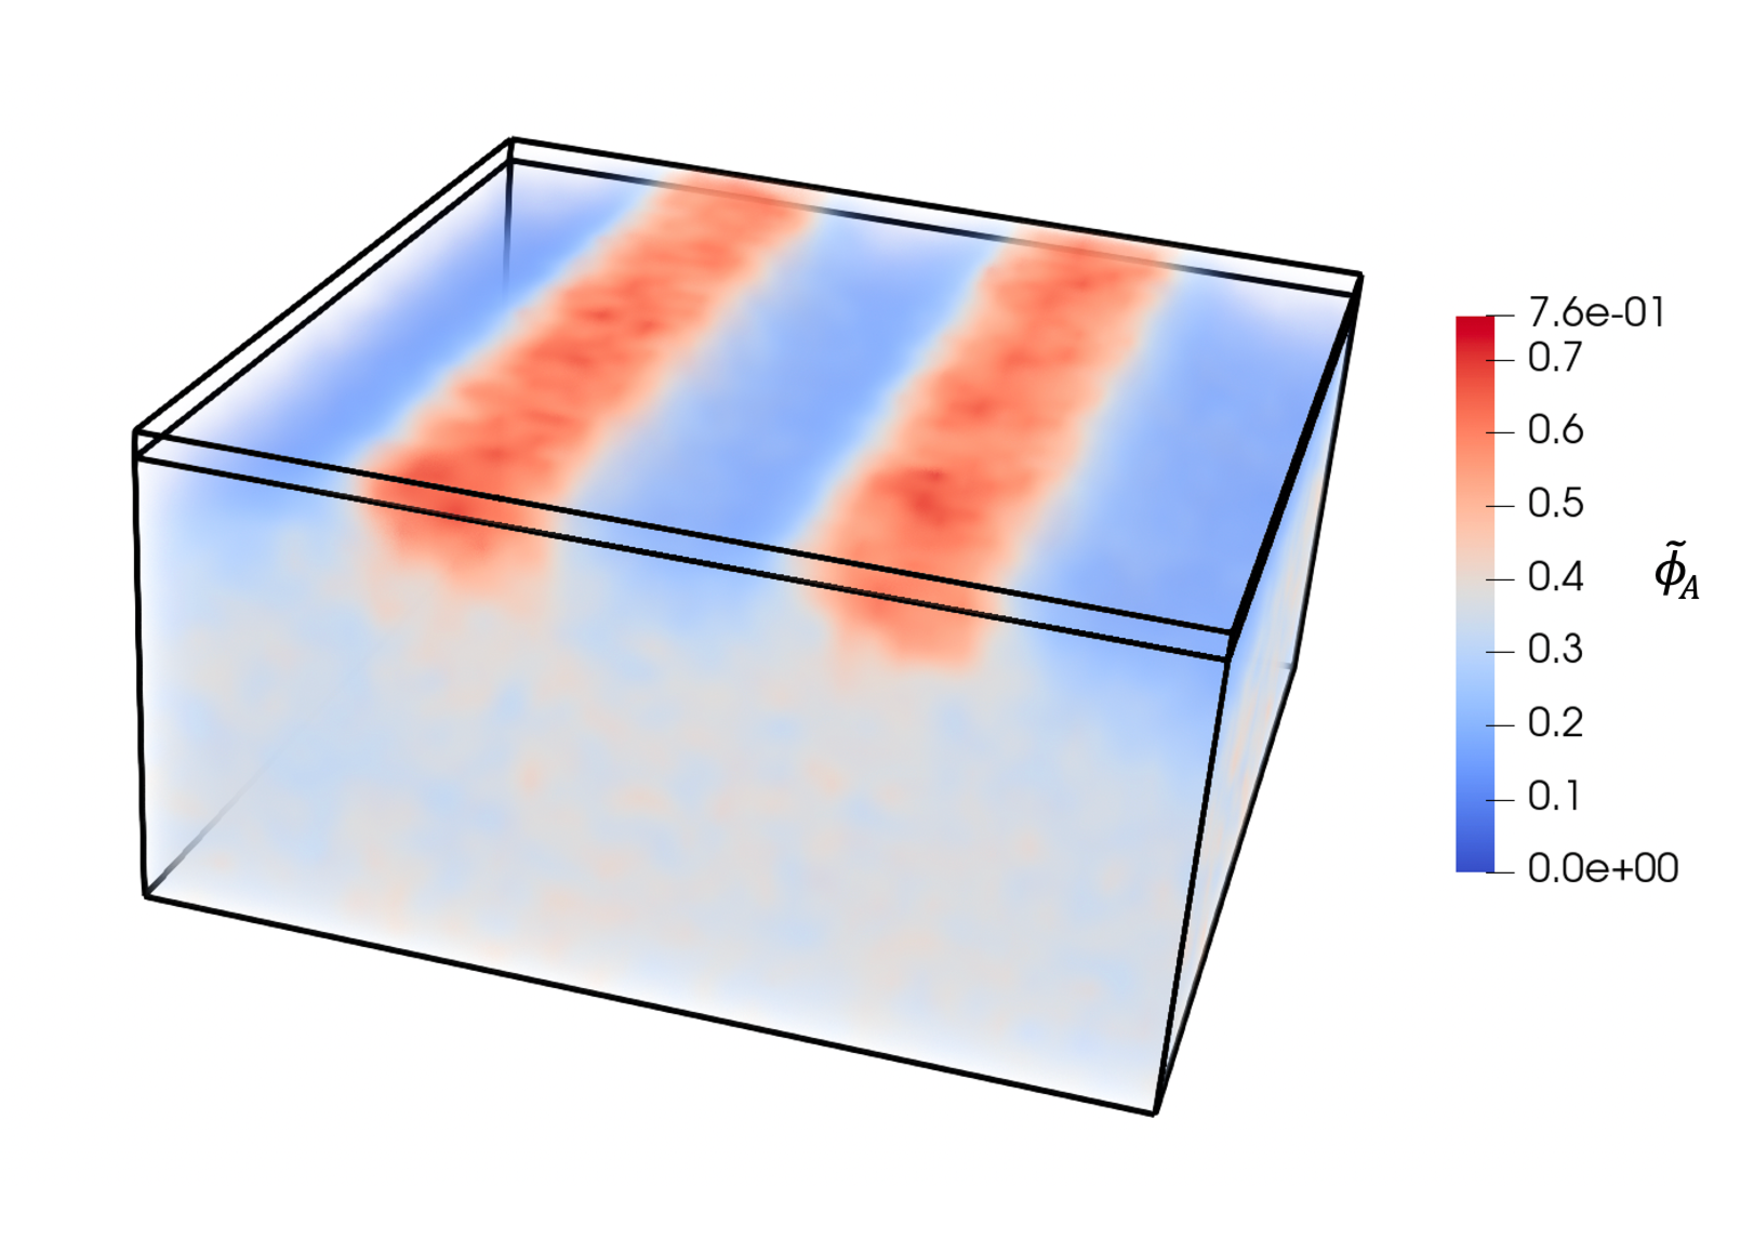
\includegraphics[width=0.5
    \linewidth]{figures/conversion_box.pdf}
    \caption{Composition $\tilde\phi_A(\mathbf r)$ after optimization for $\lambda=2\,R_e$ and $\Delta\tilde\phi=0.5\,,$ obtained using \ac{SD} algorithm. Averaged over 100 optimization runs starting from randomly generated initial configurations. The conversion zone is marked by the thin frame at the top.}
    \label{fig:conversion_box}
\end{figure}

\subsection{SA parameter choice}

As discussed previously, the performance of the \ac{SA} algorithm depends greatly on the applied temperature reduction scheme. A commonly used scheme involves \ac{LC}. The temperature in the $k$-th cycle is calculated according to

\begin{align}
    T_{k,LC}=T_0-\alpha_{LC} k\,,
    \label{eq:lin_cool}
\end{align}

where $\alpha_{LC}>0\,.$ The total number of temperature cycles is $n_{LC}=\lceil(T_0-T_{f,LC})/\alpha_{LC}\rceil\,.$ While other cooling schedules might be more efficient, \ac{LC} allows for a detailed exploration of the search space. Another option is to use an \ac{EC} schedule:

\begin{align}
    T_{k,EC}=T_0\alpha_{EC}^k\,,
    \label{eq:exp_cool}
\end{align}

where $0<\alpha_{EC}<1\,.$ This corresponds to $n_{EC}=\lceil\log_{\alpha_{EC}}(T_f/T_0)\rceil$ temperature cycles. The minimum value of the loss function at a given temperature $T$ for the different cooling schedules is denoted $L_{opt,i}(T)\,,$ with $i=LC,EC\,.$ This is shown in \autoref{fig:opt-t}a for a randomly generated initial configuration. The corresponding acceptance rate is shown in \autoref{fig:opt-t}b. The parameters are $\lambda=1.25\,R_e\,,$ $\Delta\tilde\phi=0.5\,,$ $T_0=10\,,$ $T_{f,LC}=0$ and $T_{f,EC}=10^{-4}$ . As a reference, the \ac{SD} result is also shown. With both cooling schedules, the \ac{SD} level is reached only for temperatures $T<0.1<<T_0\,.$ However, the acceptance rate already displays a significant sensitivity to temperature decrease at much larger temperature scales. The maximum temperature is therefore chosen appropriately. The final value $L_{opt,LC}(0)/n_tn_T\sigma_0^2$ decreases with $\alpha_{LC}$ before it becomes constant at a critical value $\alpha^*_{LC}\approx 10^{-5}\,.$ The results for \ac{EC} follow very similar trends. $L_{opt,EC}(0)/n_tn_T\sigma_0^2$ decreases as $\alpha_{EC}$ is increased until a critical value $\alpha^*_{EC}\,.$ The final numerical values of \ac{LC} and \ac{EC} are in exact agreement for $\alpha_{LC}\leq \alpha^*_{LC}$ and $\alpha_{EC}\geq \alpha^*_{EC}$. This is a strong indicator that the \ac{SA} algorithm successfully finds the global minimum of \autoref{eq:lossfunction} for the given initial configuration. The difference in efficiency between the two cooling schedules is substantial: for $\alpha_{LC}=10^{-5}\,,$ the \ac{LC} schedule requires $10^6$ temperature cycles, while the \ac{EC} schedule only requires about $10^{5}$ cycles to give the same value at $\alpha_{EC}=0.9999\,.$ 


\begin{figure}[H]
\centering
\begin{subfigure}[b]{\textwidth}
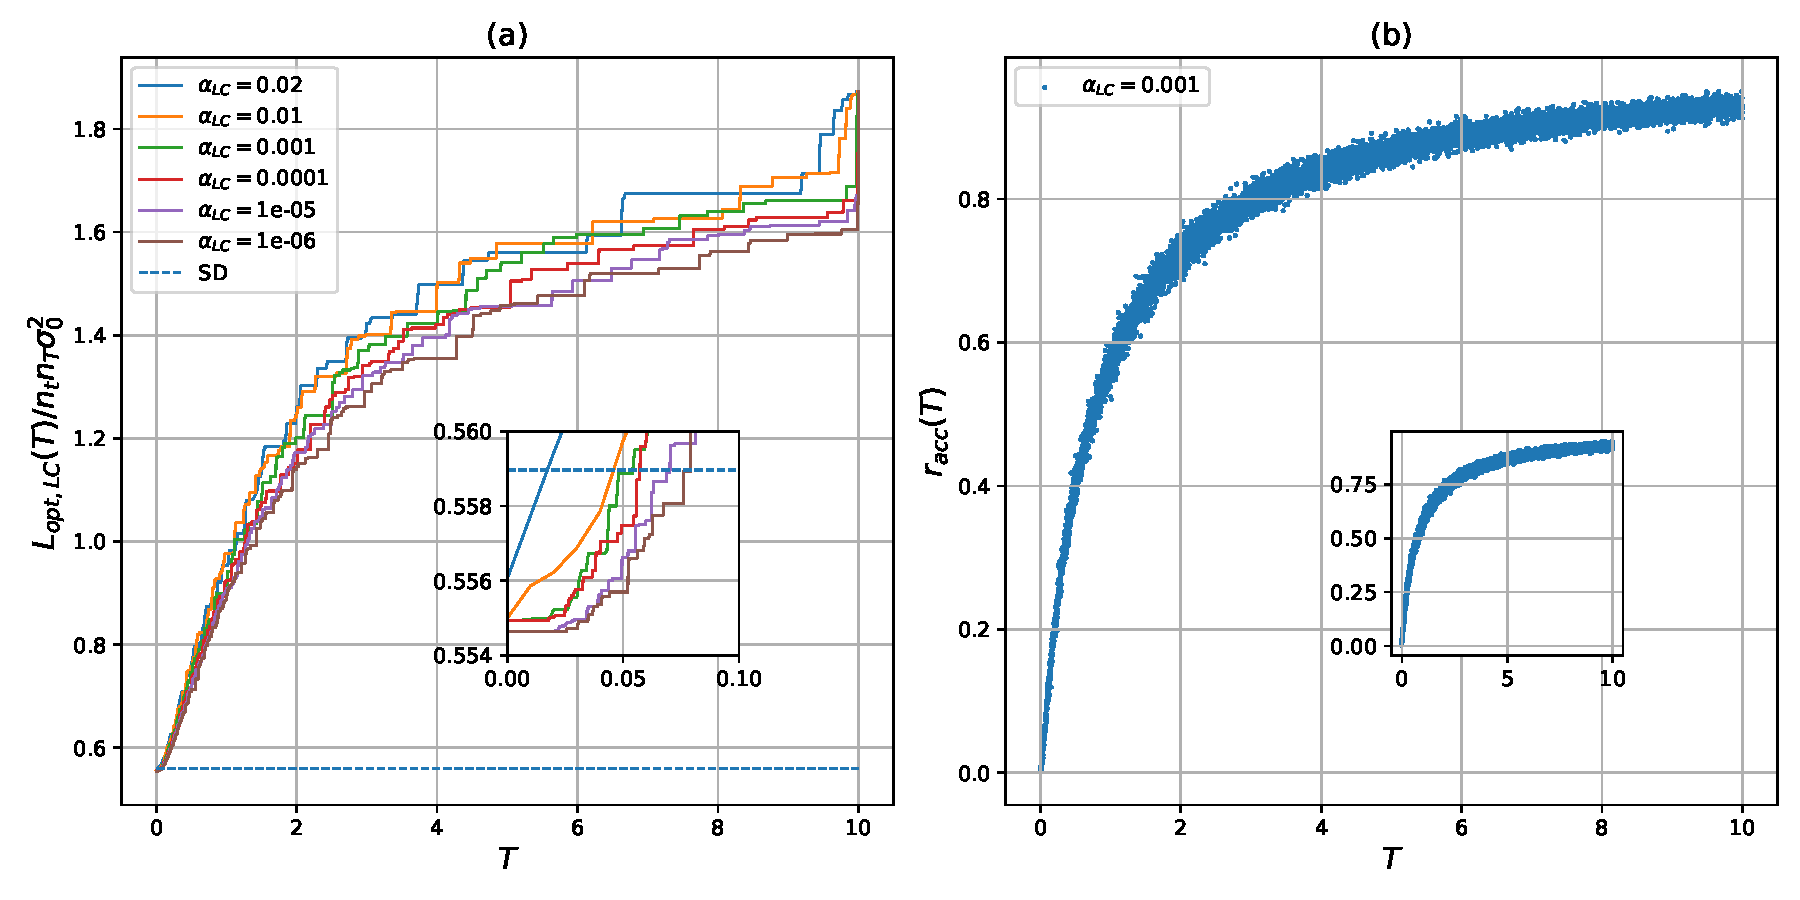
\includegraphics[width=1\linewidth]{figures/opt_T_lam1p25_dphi0.5_seed0_lin_cool.pdf}
   \label{fig:opt-t-lin-cool} 
\end{subfigure}

\begin{subfigure}[b]{\textwidth}
   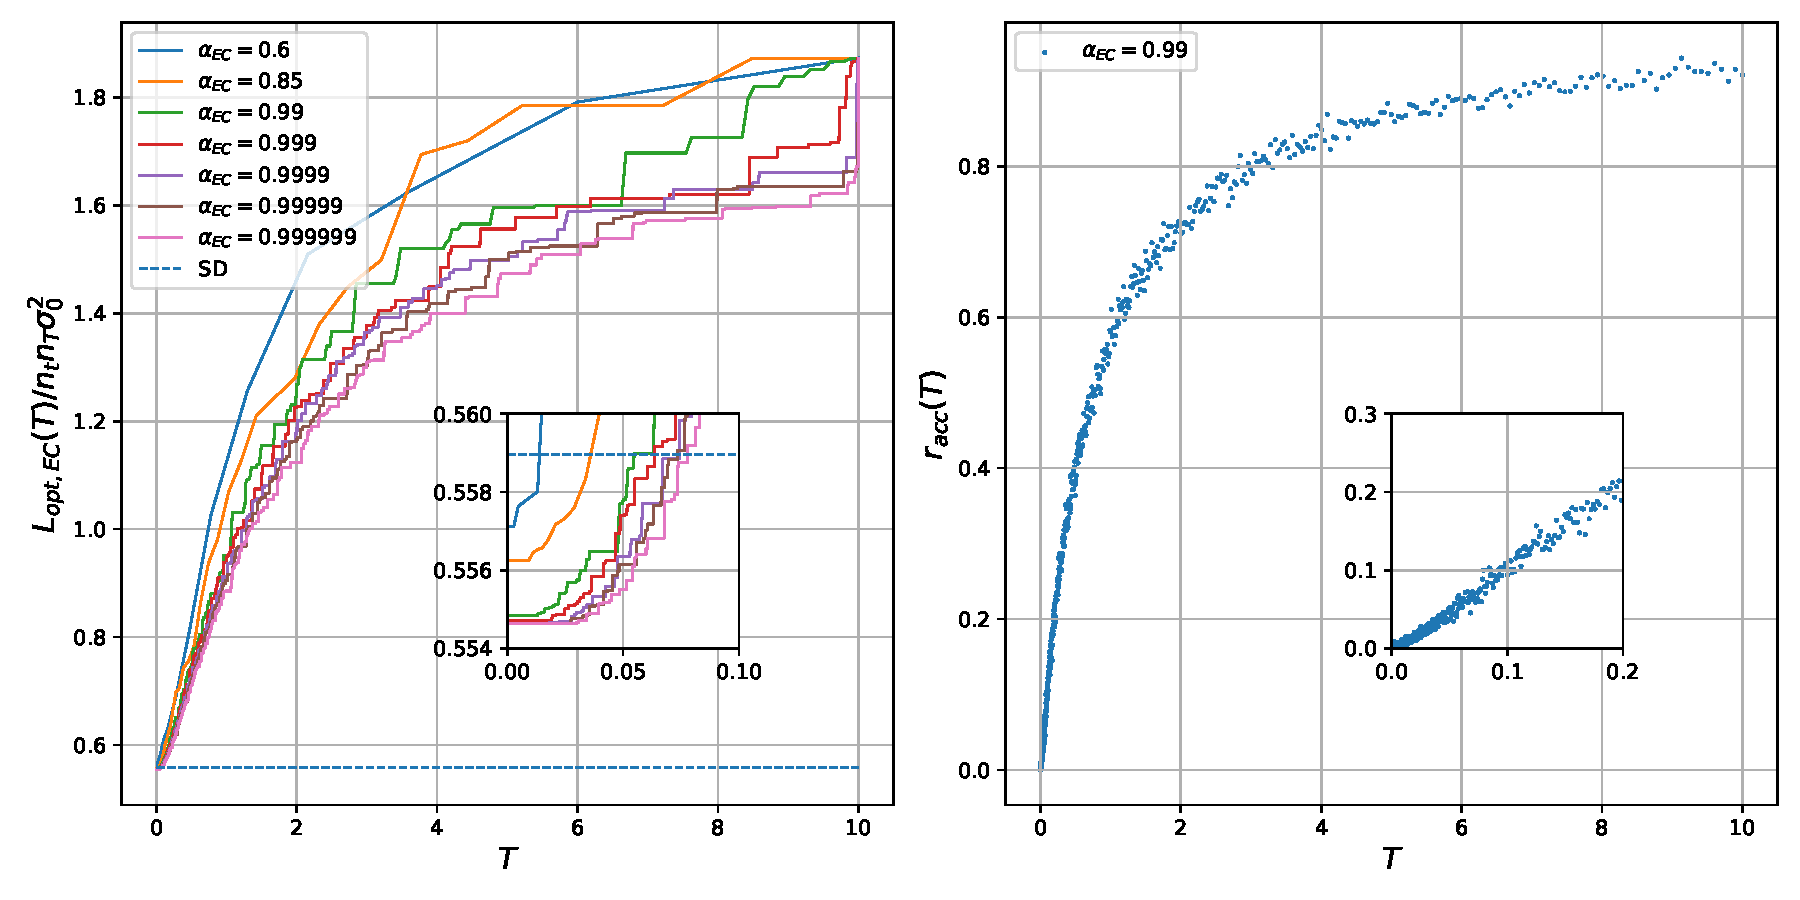
\includegraphics[width=1\linewidth]{figures/opt_T_lam1p25_dphi0.5_seed0_exp_cool.pdf}
   \label{fig:opt-t-texp-cool}
\end{subfigure}
\caption{(a) Optimum of loss function $L_{opt,i}/n_tn_T\sigma_0^2$ as a function of $T$ for several values of $\alpha_i\,.$ (b) \ac{SA} acceptance rate $r_{acc}$ as a function of $T\,.$ The top shows the results for $i=\,$\ac{LC}, the bottom for $i=\,$\ac{EC}. The insets show a section that is zoomed in to small temperatures.}
\label{fig:opt-t}
\end{figure}

The crossover of the \ac{SA} curve below the \ac{SD} level happens at a certain temperature $T^*\,,$ which depends on $\alpha_i\,.$ This temperature is important since it defines a scale of typical \enquote{energy barriers} that the \ac{SD} algorithm cannot overcome. \autoref{fig:delta_loss_hist} shows the distribution of the change in the loss function $\Delta$ for a single flip for different temperatures. For $T=10\,,$ the distribution is symmetric, which indicates that a flip may increase or decrease the value of the loss function with the same probability. As $T$ is decreased, less \enquote{good} flips are available, so the distribution becomes skewed to the right. For $T=0.06\,,$ this skew is almost complete.




\begin{figure}[h]
    \centering
    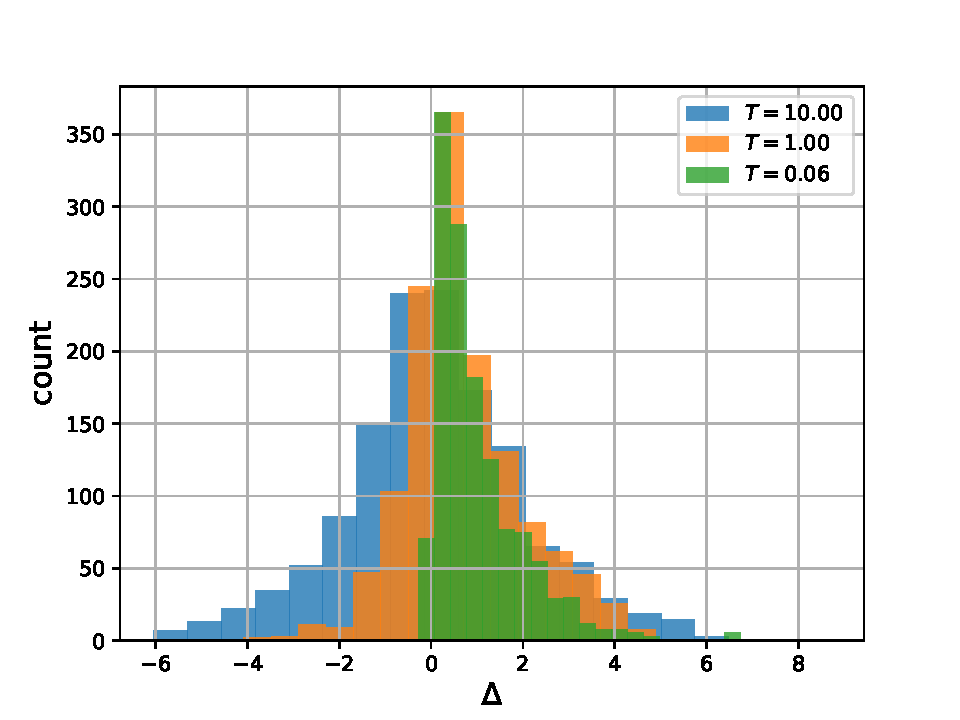
\includegraphics[width=\textwidth]{figures/delta_loss_hist_ec.pdf}
    \caption{Distribution of loss function change $\Delta$ per flip attempt at different values of $T\,.$ \ac{EC} with $\alpha_{EC}=0.999\,.$}
    \label{fig:delta_loss_hist}
\end{figure}


The improvement that \ac{SA} brings compared to \ac{SD} is very small. Although there is no way to prove that \ac{SA} finds the global minimum, it is reasonable to assume that the final value is at least close. For the investigated cases, the optimum obtained with \ac{SA} is less than $0.01\sigma_0^2$ smaller than the \ac{SD} level. This raises the question of whether \ac{SA} is even necessary, despite the obvious non-convexity of the problem. The optimized composition profiles $\tilde\phi_A(x)$ are shown in \autoref{fig:amplitude_sa_sd_lam1.25} for $\lambda=1.25\,R_e$ and in \autoref{fig:amplitude_sa_sd_lam0.25} for $\lambda=0.25\,R_e$. The \ac{SA} values are obtained from \ac{EC} with $\alpha_{EC}=0.999\,.$ The profiles obtained with the different algorithms look very similar. No tendency of the \ac{SA} profile to match the target profile better than the \ac{SD} profile can be observed at all. To quantify how different the \ac{SA} configuration is from the \ac{SD} configuration, a distance function between two configurations of target polymer types is defined:

\begin{align}
    \mathrm{dist}(\pmb\beta,\pmb\beta^*)=1-\frac{1}{n_p}\sum_{i=1}^{n_p}\delta_{\beta_i,\beta_i^*}.
\end{align}

One finds $\mathrm{dist}(\pmb\beta_{SA},\pmb\beta_{SD}))<0.05\,,$ so less than $5\%$ of the types are changed in the \ac{SA} optimum compared to \ac{SD}.

\begin{figure}[H]
  \centering
  \begin{subfigure}[b]{0.45\textwidth}
      \centering
      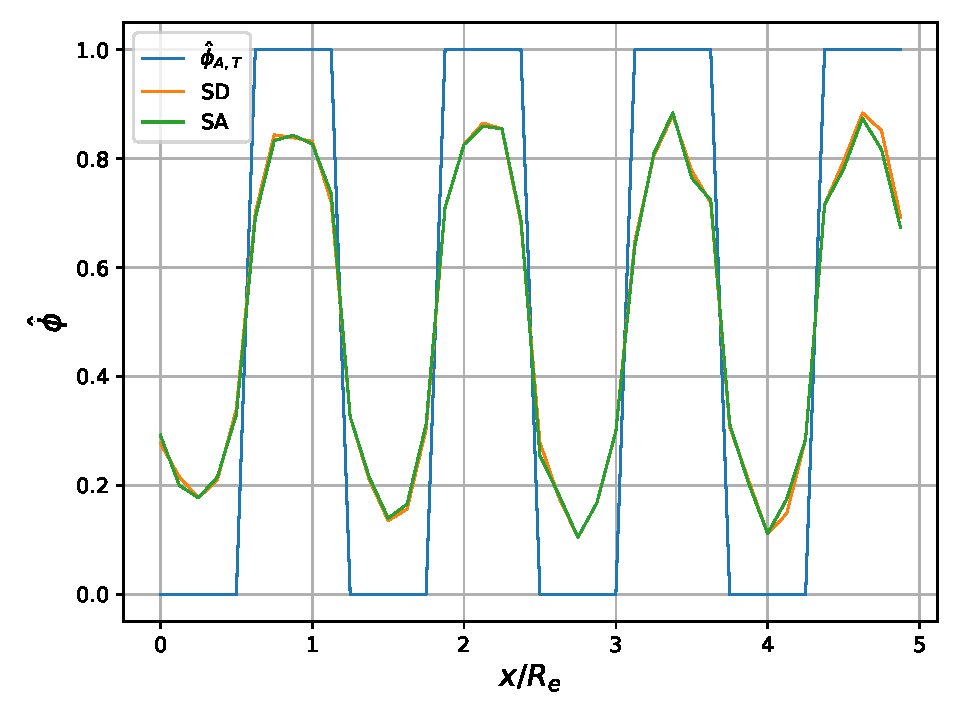
\includegraphics[width=\textwidth]{figures/amplitude_lam1p25_dphi0.5_alpha0.999_seed0.pdf}
      \caption{}
      \label{fig:amplitude_sa_sd_lam1.25}
  \end{subfigure}
    \hfill
  \begin{subfigure}[b]{0.45\textwidth}
      \centering
      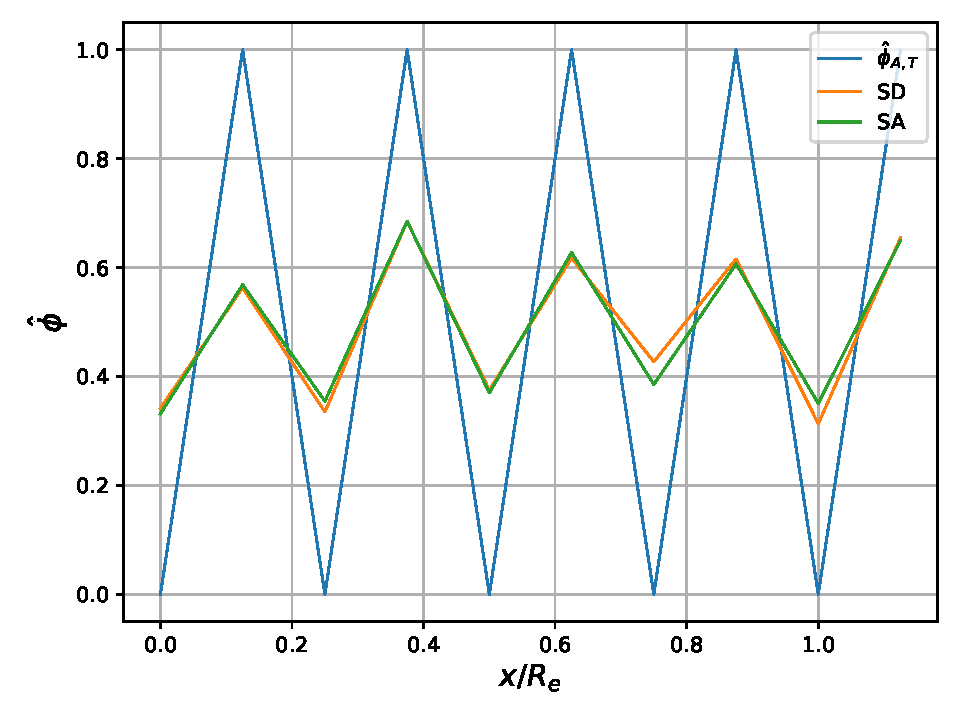
\includegraphics[width=\textwidth]{figures/amplitude_lam0p25_dphi0.5_alpha0.9999_seed0.pdf}
      \caption{}
      \label{fig:amplitude_sa_sd_lam0.25}
  \end{subfigure}
     \caption{Optimized density profile $\hat\phi_A(x)$ at $y=0\,,$ averaged over $z\,.$  The \ac{SA} curve is obtained using \ac{EC} with $\alpha_{EC}=0.9999\,.$ The target amplitude is $\Delta\tilde\phi=0.5\,.$ (a) $\lambda=1.25\,R_e\,.$ (b) $\lambda=0.25\,R_e\,.$}
     \label{fig:amplitude_sa_sd}
\end{figure}




\section{SD simulations}

In the previous section, it was concluded that the \ac{SA} algorithm does not yield significantly better results than the \ac{SD} algorithm. Additionally, while the number of flip trials performed in the \ac{SA} algorithm is fixed for a given number of target polymers and temperatures, the \ac{SD} algorithm converges faster for configurations which were recently optimized than for completely random configurations. To see this, an optimization run is performed on a randomly generated initial configuration and the number of flip proposals $n_{flips,0}$ until convergence is counted. Subsequently, a single \ac{MC} sweep is performed and the resulting configuration is optimized again, which requires $n_{flips,1}$ flip proposals. The relative difference $\Delta_{flips}=(n_{flips,0}-n_{flips,1})/n_{flips,0}$ is shown in \autoref{fig:dflips-lam} as a function of $\lambda\,,$ averaged over 100 different initial configurations.


\begin{figure}[h]
    \centering
    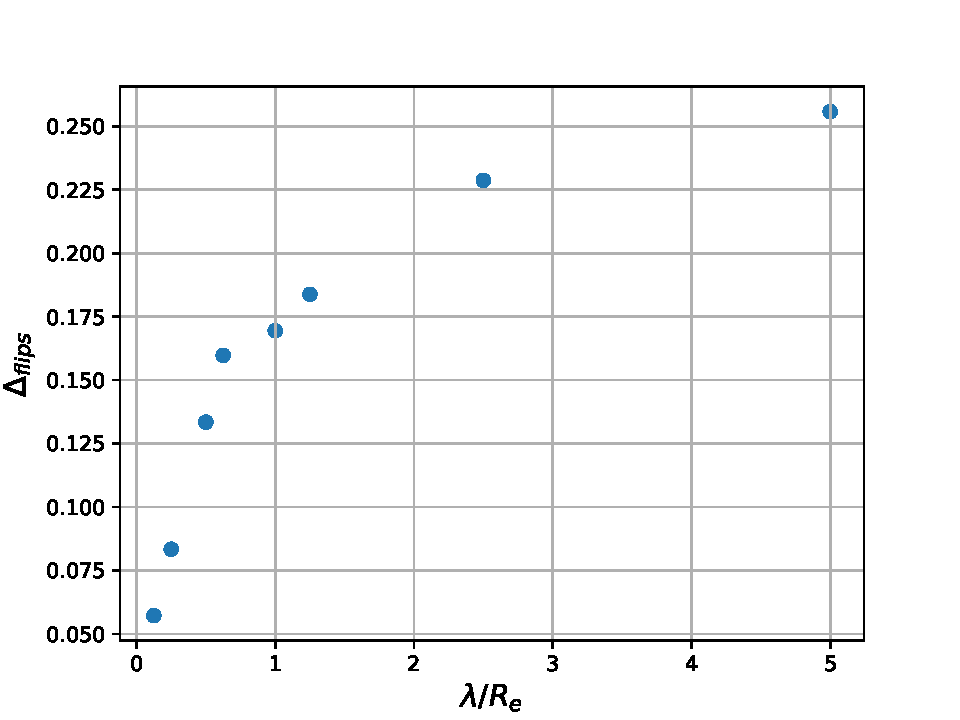
\includegraphics[width=\textwidth]{figures/dflips-lam.pdf}
    \caption{}
    \label{fig:dflips-lam}
\end{figure}


$\Delta_{flips}$ increases from about $6\%$ for $\lambda=0.25\,R_e$ to $26\%$ for $\lambda=5\,R_e\,.$ Due to this gain in efficiency, and the previously mentioned reasons, the \ac{SD} algorithm is chosen for all the following simulations.\\
One limiting factor in achieving the desired target composition is the lamella periodicity $\lambda\,.$ The optimum of the loss function is shown in \autoref{fig:L-lambda} as a function of the lamella wave vector $q=2\pi/\lambda$ for $\Delta\tilde\phi=0.5\,.$ The values of $\lambda$ are chosen such that an integer number of lamella periods fit in the simulation box. For large periodicities, the deviation of the composition from the target profile is small everywhere except in the interfacial region between the $A$-rich and the $B$-rich part. The value of the loss function then depends mainly on the number of interfaces, so one finds $L_{opt}\propto q$ for small wave vectors $qR_e/2\pi<1\,.$ For larger $q\,,$ or smaller $\lambda\,,$ finding the proper type configurations within a lamella becomes more difficult as sharp density changes are required on smaller length scales. This results in a smaller amplitude of the composition, as shown in \autoref{fig:amplitude_lamella_per} for several values of $\lambda\,.$ For $\lambda=0.5\,R_e\,,$ merely an amplitude of about $0.17$ is reached. This decrease of the amplitude explains the deviation from the linear behavior in \autoref{fig:L-lambda} for large $q\,.$ 

\begin{figure}[h]
  \centering
  \begin{subfigure}[b]{0.45\textwidth}
      \centering
      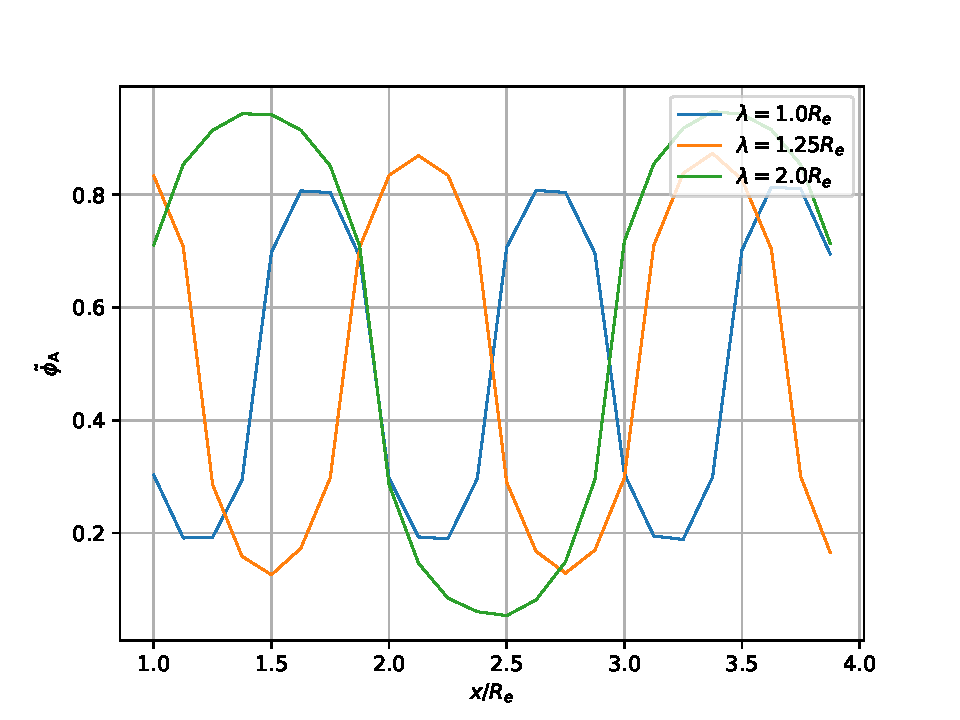
\includegraphics[width=\textwidth]{figures/amplitude_lamella_per.pdf}
      \caption{}
      \label{fig:amplitude_lamella_per}
  \end{subfigure}
    \hfill
  \begin{subfigure}[b]{0.45\textwidth}
      \centering
      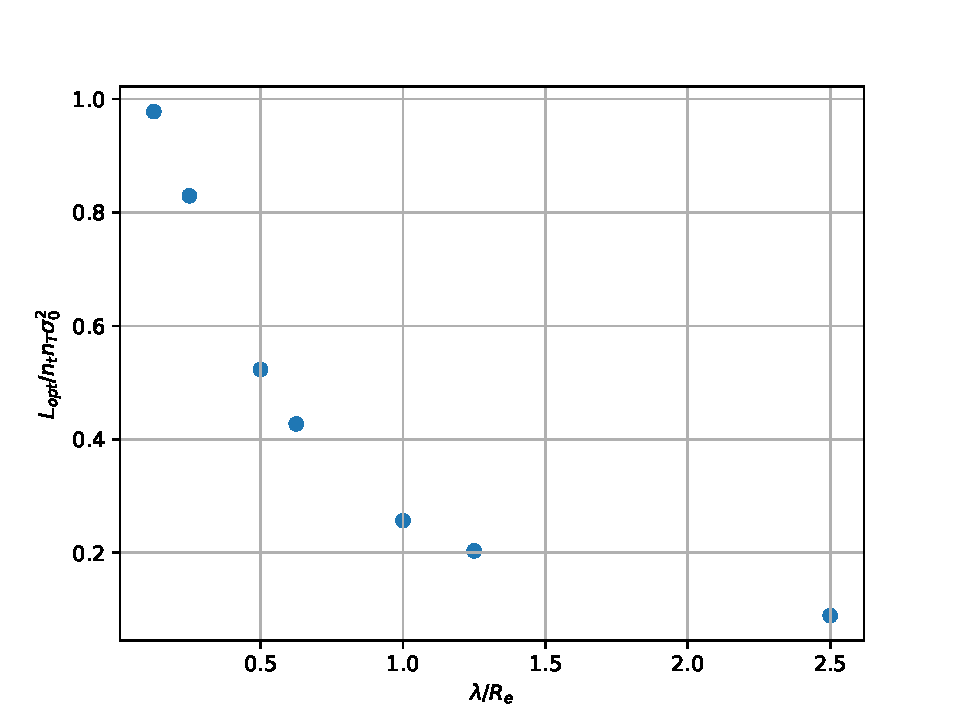
\includegraphics[width=\textwidth]{figures/L_lambda.pdf}
      \caption{}
      \label{fig:L-lambda}
  \end{subfigure}
     \caption{(a) One dimensional density profile $\hat\phi_A(x)$ at $y=0\,,$ averaged over $z\,.$ (b) Normalized loss function optimum as a function of the lamella periodicity $\lambda\,.$}
     \label{fig:periodicity-lossfunction}
\end{figure}

The large deviations of the composition profiles from the target composition, especially for small $\lambda\,,$ is not surprising, since the lamellar assembly of noninteracting homopolymers with sharp boundaries is entropically highly disfavored and the chain configurations are thus poorly suited for such target profiles. For polymers with $\chi N\neq 0\,,$ on the other hand, dictating sharp boundaries on small length scales might be desirable. For this, it is necessary to also allow the particle positions to relax.

\subsection{Impact on bulk}

Another issue caused by the finite chain-extension is the extent to which the density is influenced outside the target cells, this can already be seen in \autoref{fig:conversion_box}. The composition profile is shown in \autoref{fig:amplitude_decay_profile} for several values of $y\,.$ \autoref{fig:amplitude_decay} shows the maximum composition $\tilde\phi_{A,\mathrm{max}}$ as a function of $y\,.$ It reaches the homogeneous value of $0.5$ at a distance of about $1R_e$ from the conversion zone, as one would expect. 

\begin{figure}[h]
  \centering
  \begin{subfigure}[b]{0.45\textwidth}
      \centering
      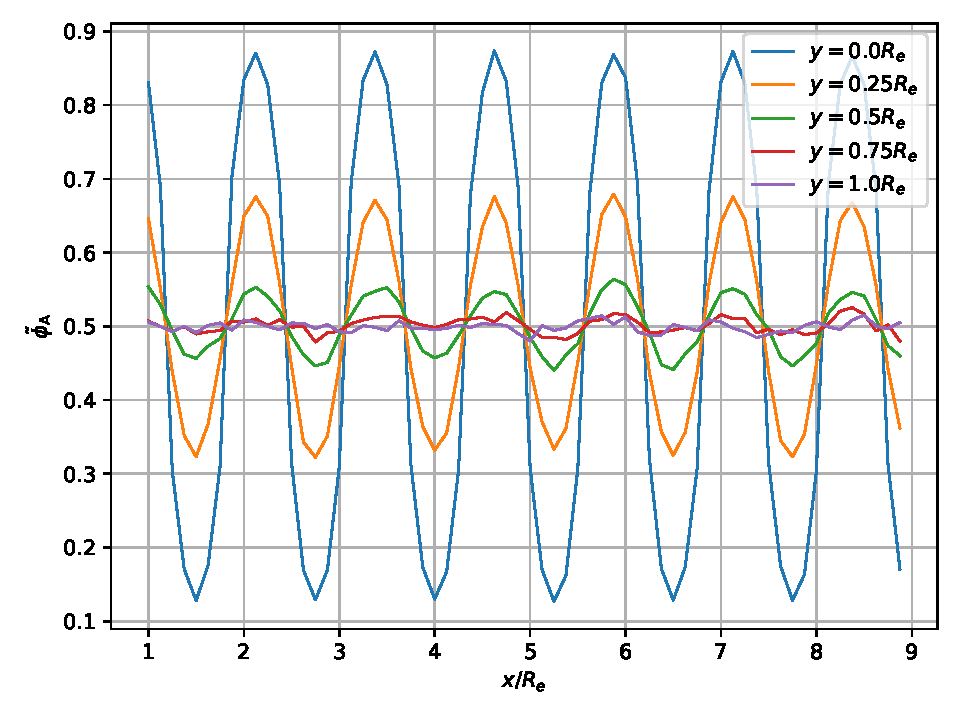
\includegraphics[width=\textwidth]{figures/amplitude_decay_profile.pdf}
      \caption{}
      \label{fig:amplitude_decay_profile}
  \end{subfigure}
    \hfill
  \begin{subfigure}[b]{0.45\textwidth}
      \centering
      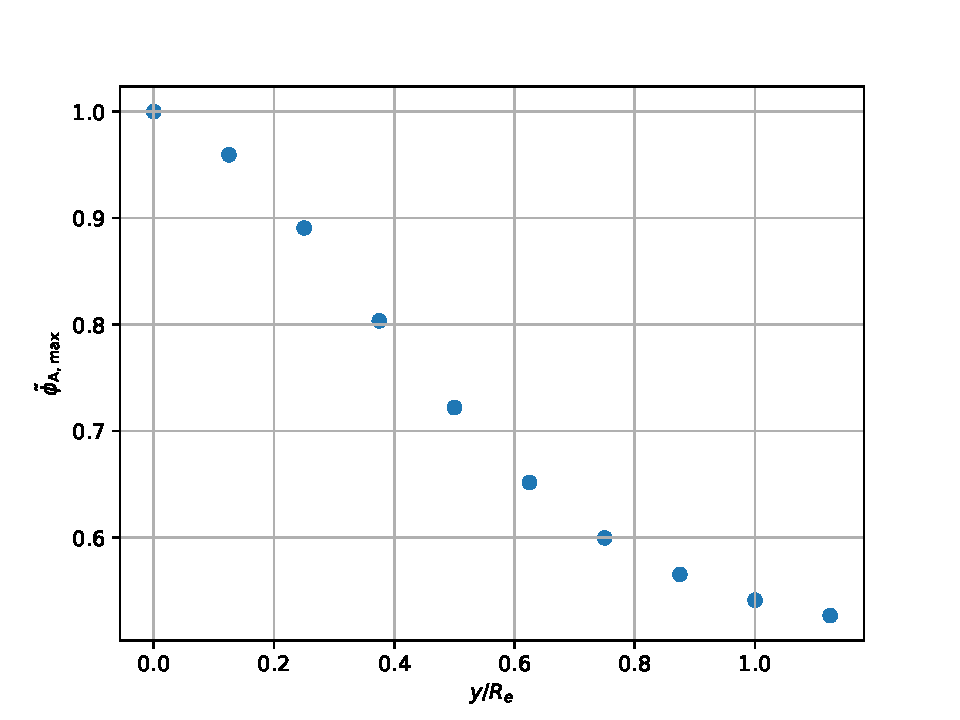
\includegraphics[width=\textwidth]{figures/ampltitude_decay.pdf}
      \caption{}
      \label{fig:amplitude_decay}
  \end{subfigure}
     \caption{(a) 1D density profile of type $A$ for various values of $y\,.$ (b) Density amplitude as a function of $y\,.$}
     \label{fig:conversion_range_bulk}
\end{figure}

\section{Hybrid strategy}
\label{sec:hybrid}

The approach to impose a target composition based only on the type-switching of polymers is flawed and the results are not satisfactory. However, it brings the unique advantage of making the system grand canonical, which is required to simulate the setting described in \autoref{fig:continuum_section}. We, therefore, want to modify this approach to better match the target composition. One way to do this would be the use of external fields, as in the previous chapter. In a more physical approach, the interaction part of the quasi-instantaneous fields \autoref{eq:calc_omegafields} is modified for the target cells:

\begin{align}
    \omega^{inter}_{A,T}(c)=-\frac{\chi N}{2}\left(\tilde\phi_{A,T}(c)-\tilde\phi_{B,T}(c)\right)\,,
    \label{eq:omega_fields_hybrid}
\end{align}

and similarly for $\omega^{inter}_{B,T}(c)\,.$ The new term involves the interaction between the target fields instead of the actual fields. The hybrid scheme now consists of an optimization run using the \ac{SD} algorithm, followed by a fixed number $\Delta MCS$ of simulation steps employing the modified fields \autoref{eq:omega_fields_hybrid}. For $\chi N\neq 0\,,$ this allows the chains to relax after the conversions have taken place.

% \subsection{Reference system}

% A system of $n=5000$ homopolymers with $N_A=N_B=N=32$ and $\chi N=0$ is used. The box dimensions are $L_x\times L_y\times L_z=5\times1\times5\,R_e^3\,,$ so $\sqrt{\bar{N}}=200\,.$ Space is discretized with $\Delta L=1/8\,R_e$ in all directions. Impenetrable walls are applied at the boundaries. For the cells directly behind the wall at $y=0\,,$ target compositions are applied.

% \subsection{Lamellar target composition}

% In this section, target compositions are applied with a lamellar periodicity, similar to the external fields in \autoref{fig:fext}. Values alternate between $0.0$ and $1.0$ for type A and vice versa for type B (\textbf{Maybe put some here}). The optimum value of $L\,,$ normalized by the number of target cells $n_T$ and the number of monomer types $n_t\,$, is shown in \autoref{fig:lamella_opt} for the hill-climbing algorithm and for the SA algorithm with a linear and an exponential cooling scheme.

% \begin{figure}[h]
%     \centering
%     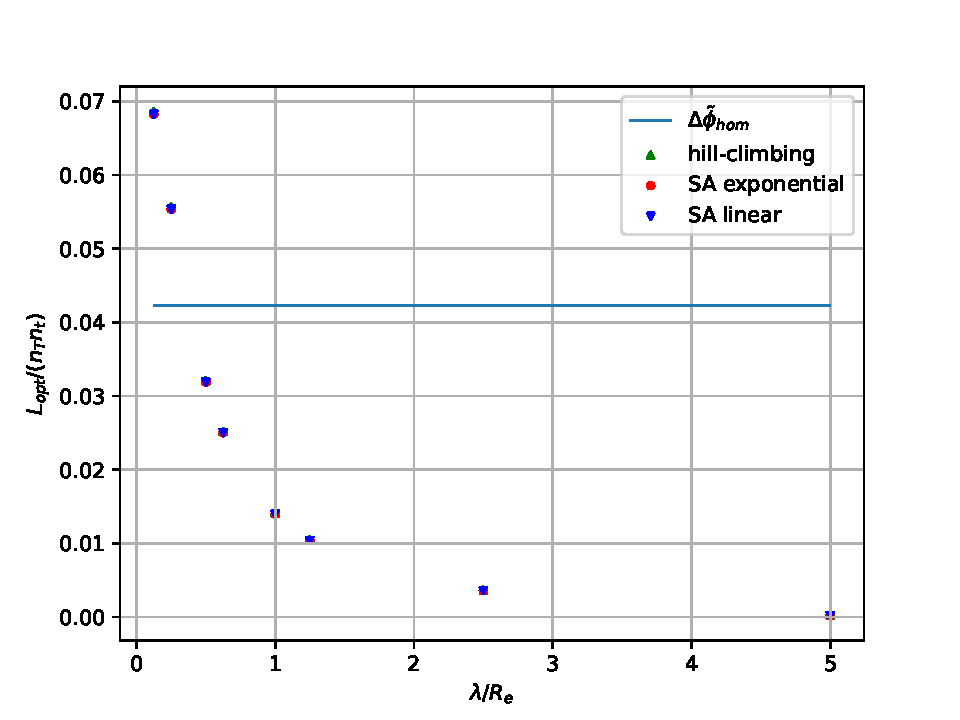
\includegraphics[width=0.6\linewidth]{figures/lamella_opt.pdf}
%     \caption{Minimum of loss function as a function of the lamella periodicity for different optimization schemes, each points is averaged over 100 randomly generated initial configurations.  The initial SA temperature is set to $T_0=1.0\,.$ The exponential cooling scheme is $T_k=T_0 0.85^k$ until $T=T_f=0.001$ and the linear cooling scheme is $T_k=T_0-0.1k$ until $T=T_f=0.0\,.$ $\Delta\hat\phi_{hom}$ denotes the variance of the density at the boundaries for the homogeneous system.}
%     \label{fig:lamella_opt}
% \end{figure}

% The values corresponding to different optimization schemes are virtually indistinguishable, the SA schemes do not find a better minimum than the hill-climbing algorithm.


% \subsection{Checkerboard-like target composition}

% \begin{figure}[h]
%     \centering
%     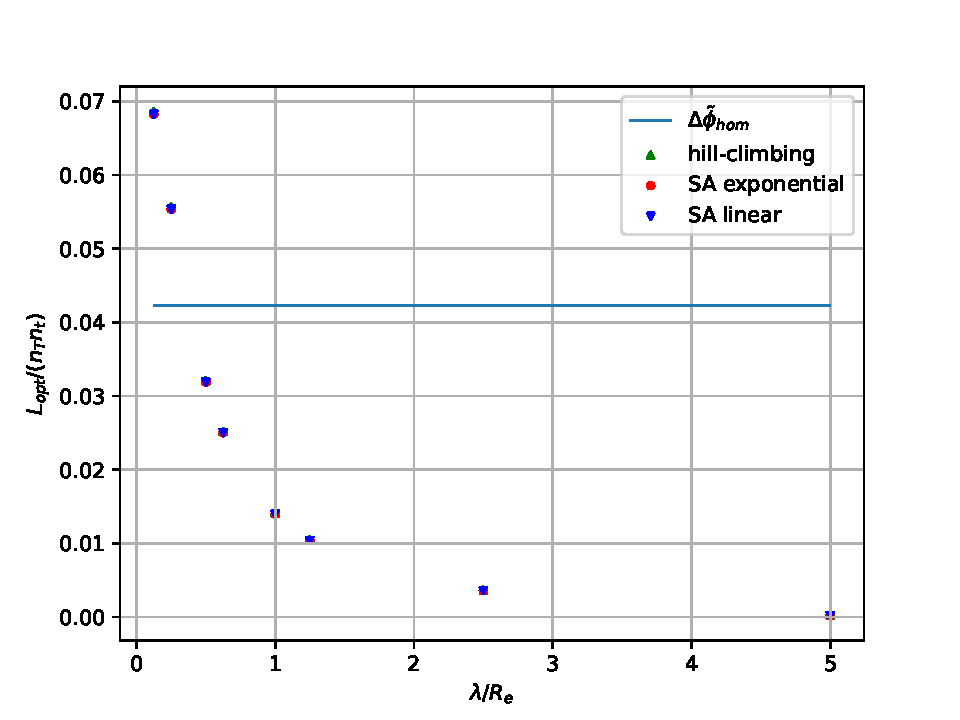
\includegraphics[width=0.6\linewidth]{figures/lamella_opt.pdf}
%     \caption{Minimum of loss function as a function of the checkerboard periodicity for different optimization schemes, each points is averaged over 100 randomly generated initial configurations.  The initial SA temperature is set to $T_0=1.0\,.$ The exponential cooling scheme is $T_k=T_0 0.85^k$ until $T=T_f=0.001$ and the linear cooling scheme is $T_k=T_0-0.1k$ until $T=T_f=0.0\,.$ $\Delta\hat\phi_{hom}$ denotes the variance of the density at the boundaries for the homogeneous system.}
%     \label{fig:checkerboard_opt}
% \end{figure}

% \newpage
% \section{Structure factor}

% \begin{itemize}
%     \item From here on, only use SD algorithm
%     \item target composition over whole system, compare collective structure factor before and after optimization
% \end{itemize}

% The collective structure factor is \cite{Reister02}:

% \begin{align}
%     S_\text{coll}(\mathbf q)=\rho_0\int_Vd^3\mathbf r\exp(i\mathbf{qr})P_\text{coll}(\mathbf r)\,,
% \end{align}
 
% where $P_\text{coll}(\mathbf r)$ is the auto-correlation of the density:

% \begin{align}
%     P_\text{coll}(\mathbf r)=\langle\phi(\mathbf x)\phi(\mathbf x +\mathbf r)\rangle_{\mathbf{x}}\,,
% \end{align}
 
% where $\mathbf{r}$ is the separation vector, $\mathbf x$ is the position and $\langle .\rangle_\mathbf x$ denotes the ensemble average.

\chapter{Summary}

\section{Collective diffusion}

The key result is that the collective dynamics of homopolymers in a quasi grand-canonical ensemble are accurately described by the simple Onsager coefficient given by \autoref{eq:onsager}. This leads to a standard diffusion equation \autoref{eq:diffusion}, which involves only the density of species $A$ and the single chain diffusion coefficient $D\,.$ This essentially means that the system can be considered an ideal gas of polymer chains. While this is partially an artifact of the similarities between the Flory-Huggins theory and regular solution theory, it is surprising that the assumption of local-coupling of the Onsager coefficient, which completely ignores the chain connectivity, gives the correct results.

\section{External field driven flow}

A simple way to implement time-dependent boundary conditions using external fields is presented in this thesis. This method is leveraged to drag lamellar layers of diblock-copolymers through the simulation box, causing them to deform under the experienced friction force. A P\'eclet number $P_e$ is defined, which describes the ratio between convective and diffusive motion. At a critical number of $P_e\approx 0.85\,,$ the lamellae break. Furthermore, the description of the system is completely analogous to a solid beam bending under a uniform load in the Euler-Bernoulli theory. This is exploited to obtain the bending modulus $K$ of the lamellae. It is found that $K$ increases as $N$ is increased, which would mean that, for a finer chain discretization, more energy is required per unit length to deform the lamellae. This is highly unexpected and may result from a scaling error of the diffusion constant in the \ac{SCMF} simulations. For $N\rightarrow\infty\,,$ one would expect the value to approach the \ac{SCFT} value. However, $K_\text{SCFT}=0.16\,\sqrt{\bar N}k_BT/R_e$ is significantly smaller than $K_\infty=0.22\,\sqrt{\bar N}k_BT/R_e\,.$

\section{Polymer-type-conversion-based target composition}

It is shown that the problem of applying non-periodic boundary conditions based on polymer type conversions in \ac{SOMA} can be interpreted as an optimization problem for the polymer type configurations. The loss function that needs to be minimized is given by \autoref{eq:lossfunction}. Two optimization algorithms are presented: the \ac{SA} algorithm and the \ac{SD} algorithm. Their performance is compared by taking different test systems and imposing lamellar target compositions at one of the boundaries with amplitude $\Delta\hat\phi$ and periodicity $\lambda\,.$ While the minimum obtained with \ac{SA} is always slightly smaller than the one obtained with \ac{SD}, this difference does not show in the density profiles. Intuitively, it is expected that the \ac{SA} algorithm performs particularly well for \enquote{difficult} target profiles, e.g., large values of $\Delta\hat\phi$ and small values of $\lambda\,.$ While the latter is indeed observed, the improvement of the \ac{SA} algorithm actually decreases as a function of $\Delta\hat\phi\,.$ It should, however, be emphasized that, for all of the investigated cases, the difference $\Delta L_{opt}$ is too small for the \ac{SA} algorithm to actually produce a density profile that is visibly closer to the target profile than the \ac{SD} profile. It is therefore one of the key results of this thesis, that the \ac{SD} algorithm should be used as it yields virtually the same results and is computationally less expensive. \\


\chapter{Outlook}

\begin{itemize}
    \item Still the old version from Einfuehrung ins Wissenschaftliche Arbeiten
\end{itemize}

The collective diffusion coefficient of a symmetric homopolymer mixture under a boundary-driven diffusion flux has been studied. In the future, more sophisticated and time-dependent boundary conditions will be employed to manipulate the behavior of the bulk, with the ultimate goal of simulating smaller sections of a large continuum simulation using particle-based simulations. The key question is whether or not the time evolution of the boundary densities is sufficient to dictate the time-evolution of the densities in the bulk. An approach based purely on center-of-mass-based polymer conversion zones might be problematic due to the extension of the converted chains beyond the boundaries. Simple conversions without changing the position of the beads may also lead to unlikely configurations of the affected polymer, so it might be necessary to let the chain grow into the simulation box, e.g. using the configurational bias method \cite{ConfBias}.






% \cleardoublepage
%% Bibliographie. Das Argument muss der Name der BIBTeX-Datenbank stehen.
%% Ein Beispiel fuer eine solche Datenbank finden Sie in bthesis_datenbank.bib
\bibliography{bthesis_datenbank} 

% \chapter*{Danksagung}
% Dank\dots

% %% Dieser Befehl MUSS am Ende stehen und erzeugt die Erklaerung ueber die
% %% benutzten Mittel
% \Declaration
\end{document}
